%  -----------------------------------------------------------------------------
%  Author         : Bimalka Piyaruwan Thalagala
%  GitHub         : https://github.com/bimalka98
%  -----------------------------------------------------------------------------

\documentclass[a4paper,11pt]{article}%,twocolumn
\input{settings/packages}
\input{settings/page}
\input{settings/macros}
\usepackage[ framed, numbered]{matlab-prettifier}%framed,%
\usepackage{listings}
\usepackage{pythonhighlight}
\usepackage{float}
\usepackage{epstopdf}
\usepackage{pdfpages}
\usepackage[toc,page]{appendix}

\begin{document}

\begin{titlepage}
\center % Center everything on the page

%-------------------------------------------------------------------------------------
%	HEADING SECTIONS
%------------------------------------------------------------------------------------
\textbf{\large Department of Electronic and Telecommunication Engineering}\\[0.5cm]
\textbf{\Large University of Moratuwa, Sri Lanka}\\[1cm]
\textbf{\large EN3053 - Digital Communications - I}\\[2cm]
\includegraphics[width=0.3\textwidth]{figures/uomlogo}\\[2cm]

	
%-------------------------------------------------------------------------------------
%	TITLE SECTION
%------------------------------------------------------------------------------------
\textbf{\Huge Lab Assignment}\\[0.5cm]
\textbf{\Large Eye diagrams and Equalization }\\


%----------------------------------------------------------------------------------------
%	MEMBERS SECTION
%----------------------------------------------------------------------------------------
\vfill % Fill the rest of the page with whitespace

\textbf{\large Submitted by}\\[0.5cm]
\begin{minipage}{0.2\textwidth}
	\begin{flushleft}
		{\large Thalagala B.P.}\\[4mm]
		{\large Samarasinghe P.}\\[4mm]

		
		
	\end{flushleft}
\end{minipage}
\hspace{5mm}
\begin{minipage}{0.2\textwidth}
	\begin{flushright}
		{\large 180631J }\\[4mm]
		{\large 180554B }\\[4mm]

	\end{flushright}
\end{minipage}\\[1.5cm]

%----------------------------------------------------------------------------------------
%	DATE SECTION
%----------------------------------------------------------------------------------------

\textbf{\large Submitted on}\\[0.5cm]
\textbf{\Large \today} % Date, change the \today to a set date if you want to be precise

%----------------------------------------------------------------------------------------



\end{titlepage}

\tableofcontents
%\listoffigures
%\listoftables
\vfill


\begin{center}
	\textit{\textbf{Note:}}
\textit{{\tt MATLAB R2018a} of the MathWorks Inc. is used for the implementation.}
\end{center}
\pagebreak

%%-----------------------------------------------------------------------
\section{Task 1}

Please note that for the MATLAB implementation bit rate(bits/second) of the generator was assumed to be 10. As we consider BPSK for the Task 1 and 2, the symbol rate(symbols/second) is remain the same as the bit rate of the generator.

\subsection{Generation of an Impulse Train Representing BPSK Symbols}
Binary data of the generator $D \in \{0, 1\}$ is mapped in to an impulse train according to the following function where $A(Amplitude)$  of the impulse was taken as 1 in the MATLAB implementation.
\[
amplitude ~of~ the~ k^{th}~ impulse = \begin{cases}
	+A & if~ D = 1\\
	-A & if~ D = 0
\end{cases}
\]

\begin{figure}[H]
	\centering
	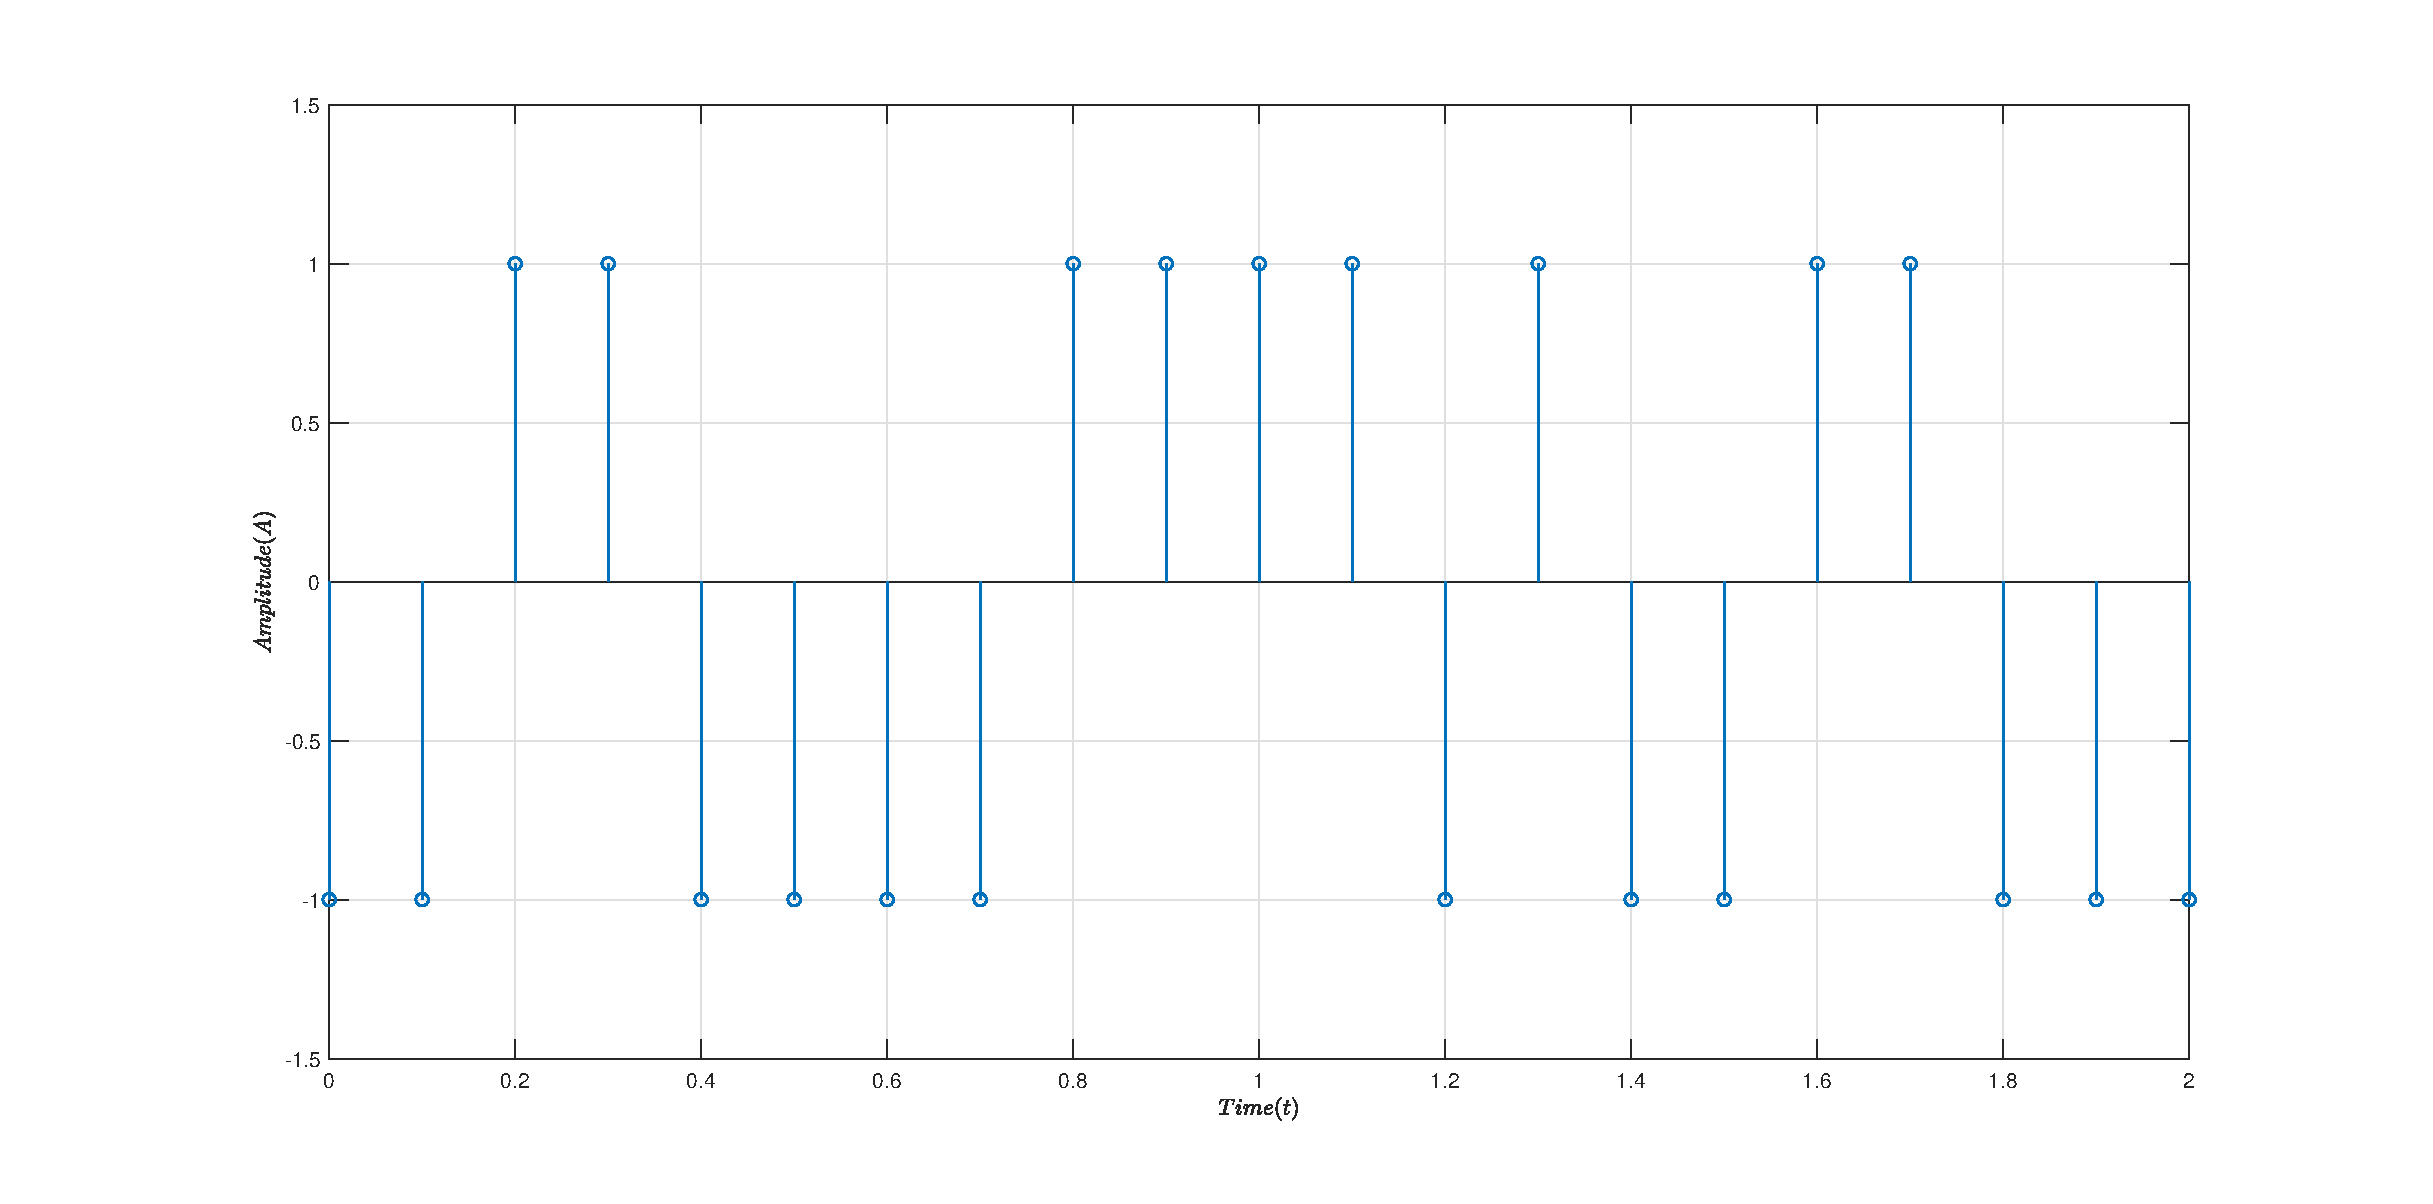
\includegraphics[scale=0.4]{figures/task11}
	\caption{Impulse Train Representing BPSK Symbols}
\end{figure}

\subsection{Transmit Signal}
\subsection{Sinc function as the Impulse response}

Function {\tt sinc(t)} in MATLAB is defined as follows. 
\[
{\tt sinc(t)} = \begin{cases}
	\frac{sin(\pi.t)}{\pi.t} & if~t \neq 0\\
	1 & if~ t = 1
\end{cases}
\]

In order to generate  a sinc pulse that aligns with our time scale the function argument should be given as mentioned below. Where $T_b$ is the separation between
successive transmitted pulses.

\[
sinc~pulse = {\tt sinc(\frac{t}{T_b})}
\]
\begin{figure}[H]
	\centering
	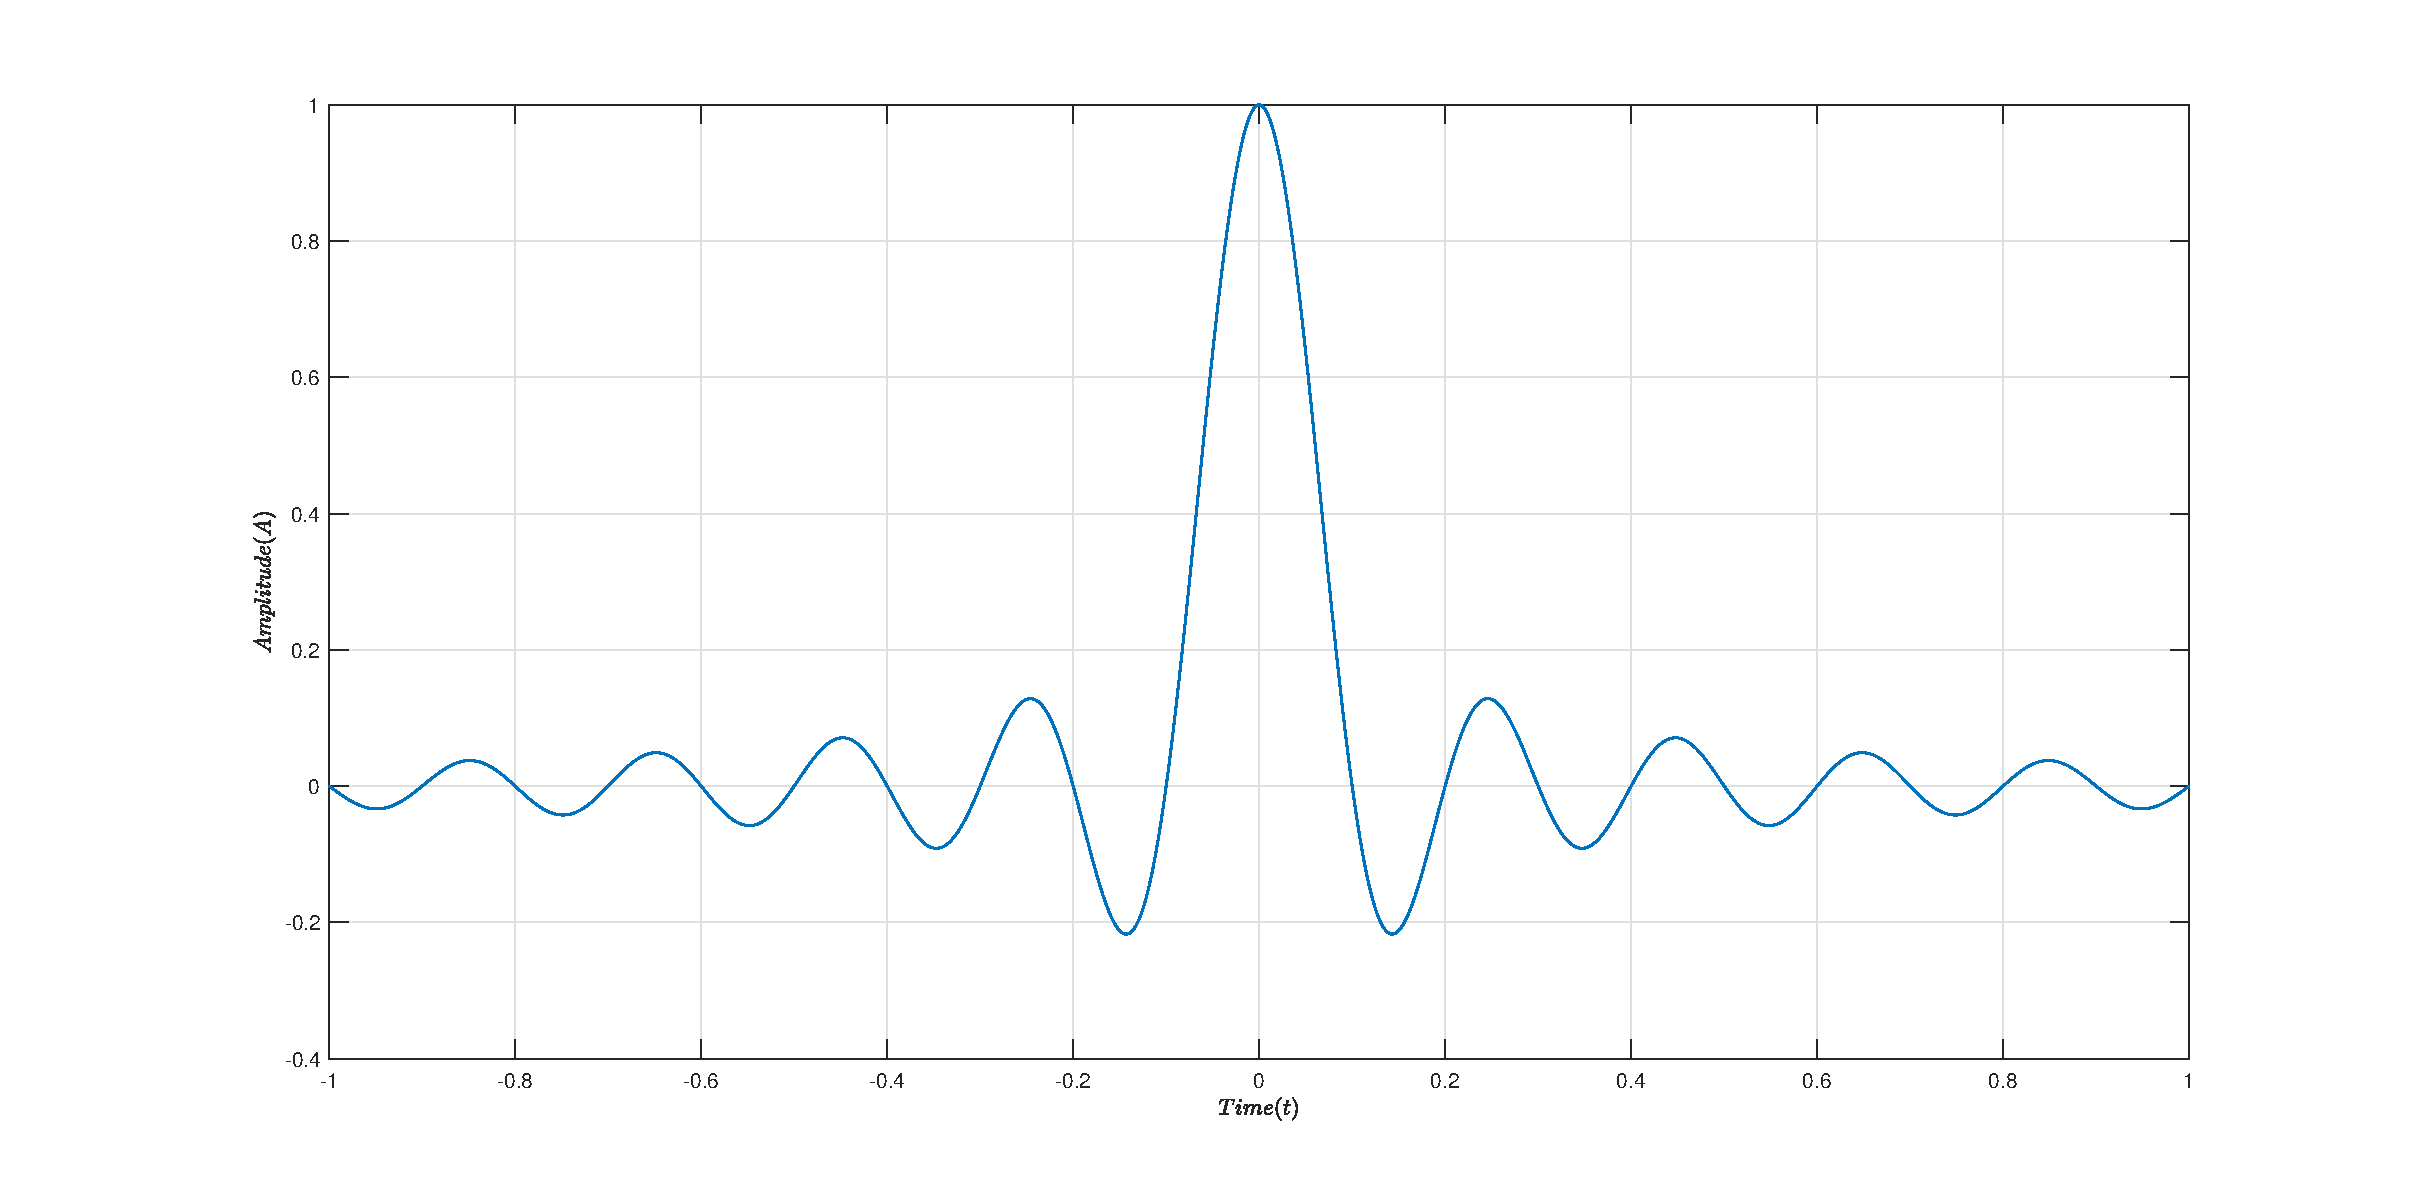
\includegraphics[scale=0.4]{figures/task12}
	\caption{Sinc function as the Impulse response of the Pulse Shaping Filter}
\end{figure}

\subsection{Convolving the Impulse train with the Sinc Pulse}

\begin{figure}[H]
	\centering
	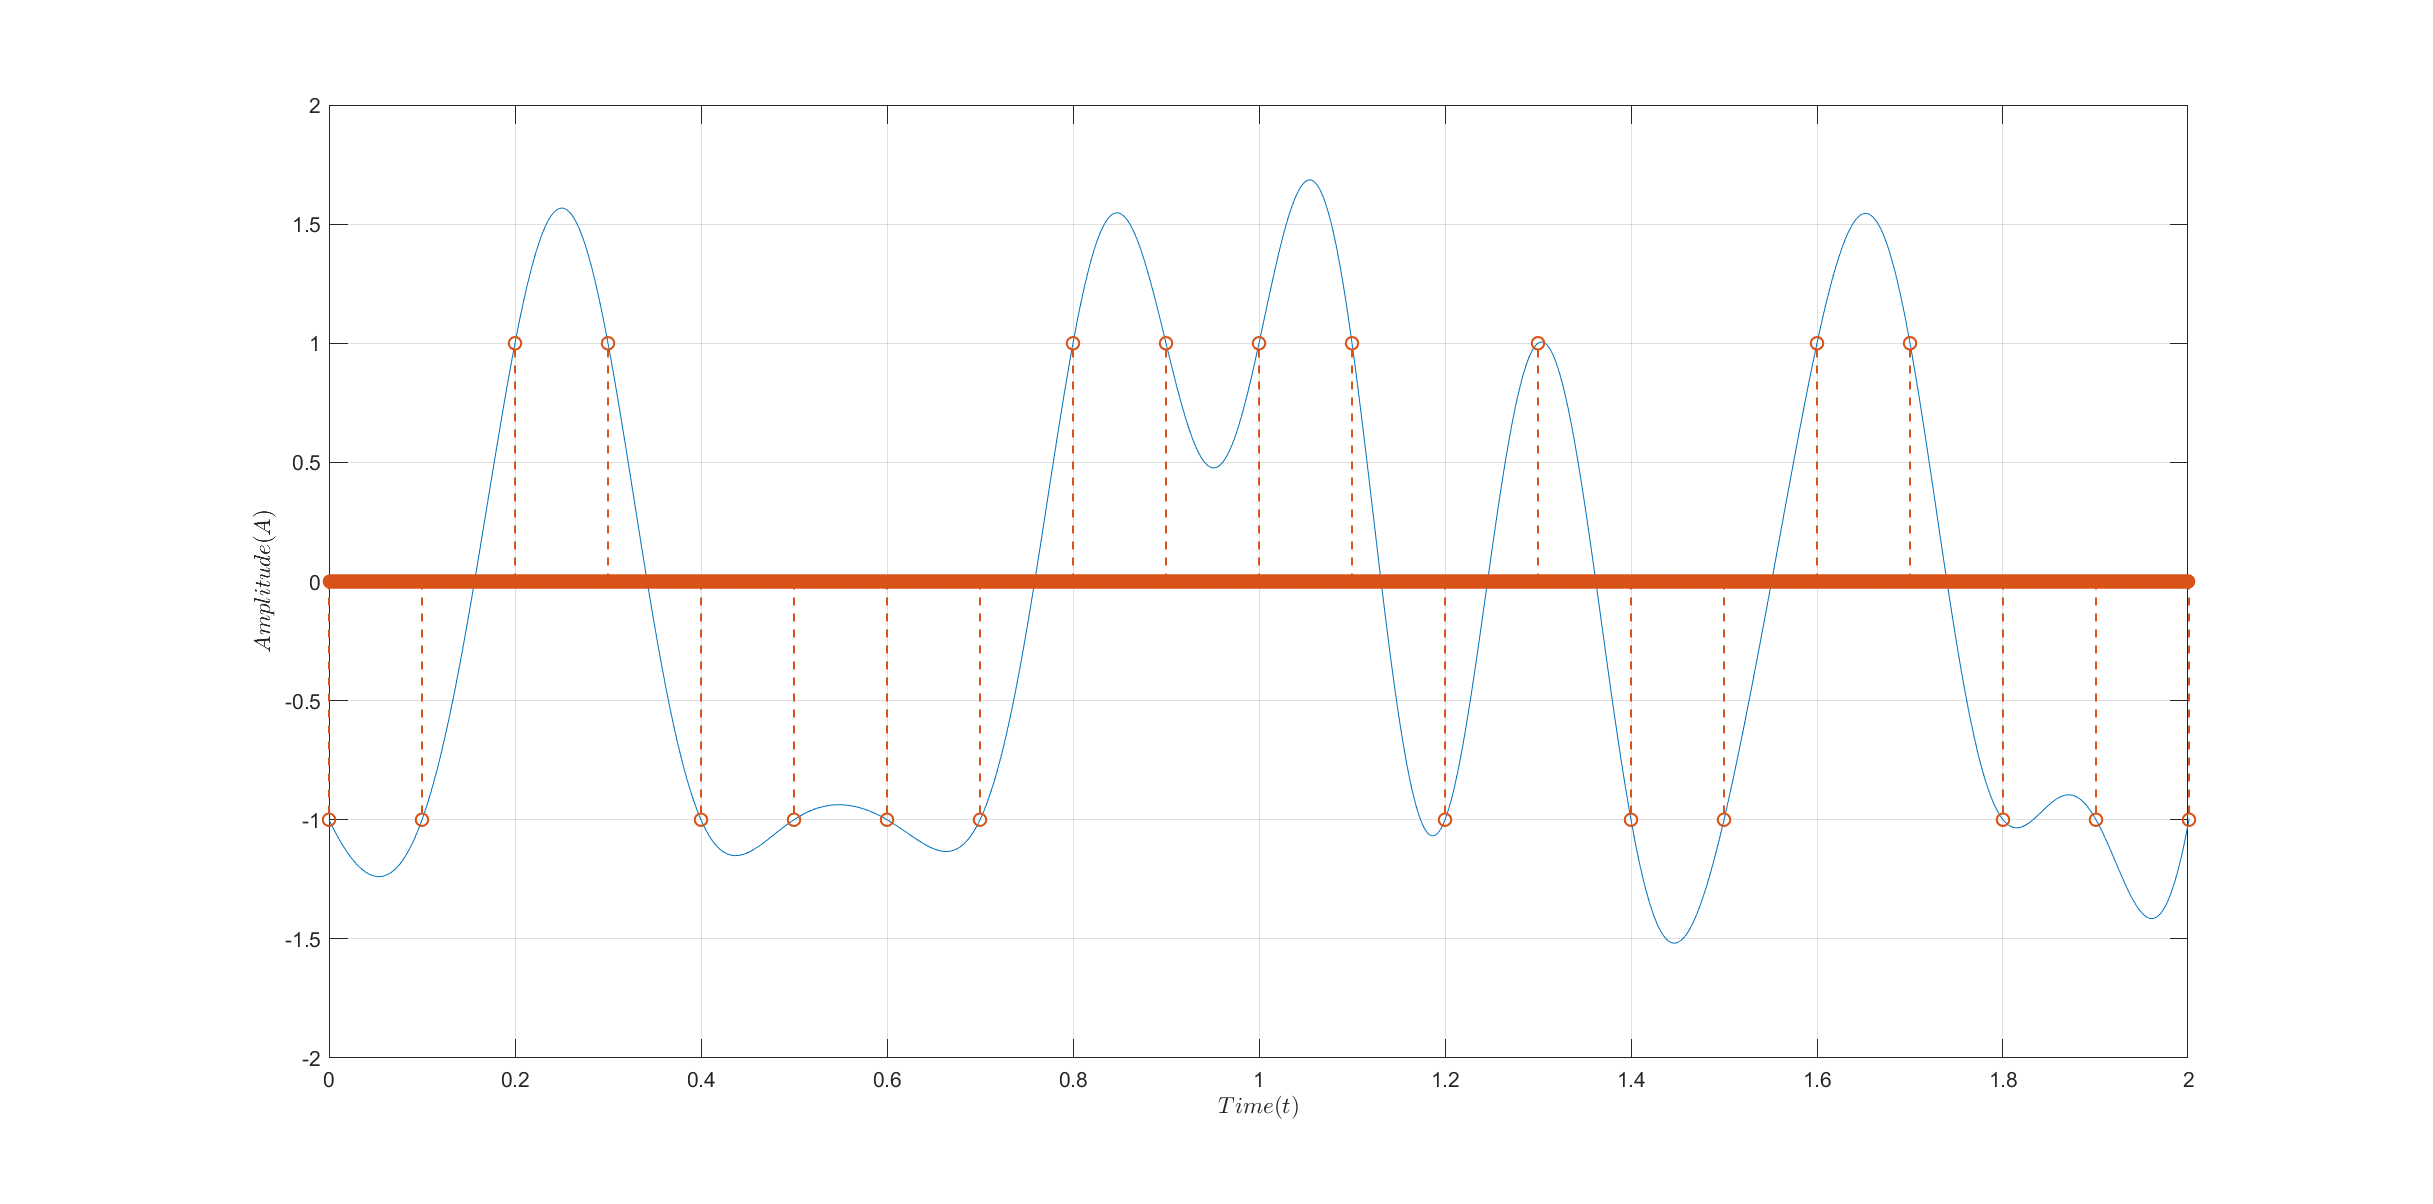
\includegraphics[scale=0.4]{figures/task14}
	\caption{Transmit Signal by Convolving the Impulse train with the Sinc Pulse}
\end{figure}

\subsection{Eye Diagram}

\begin{figure}[H]
	\centering
	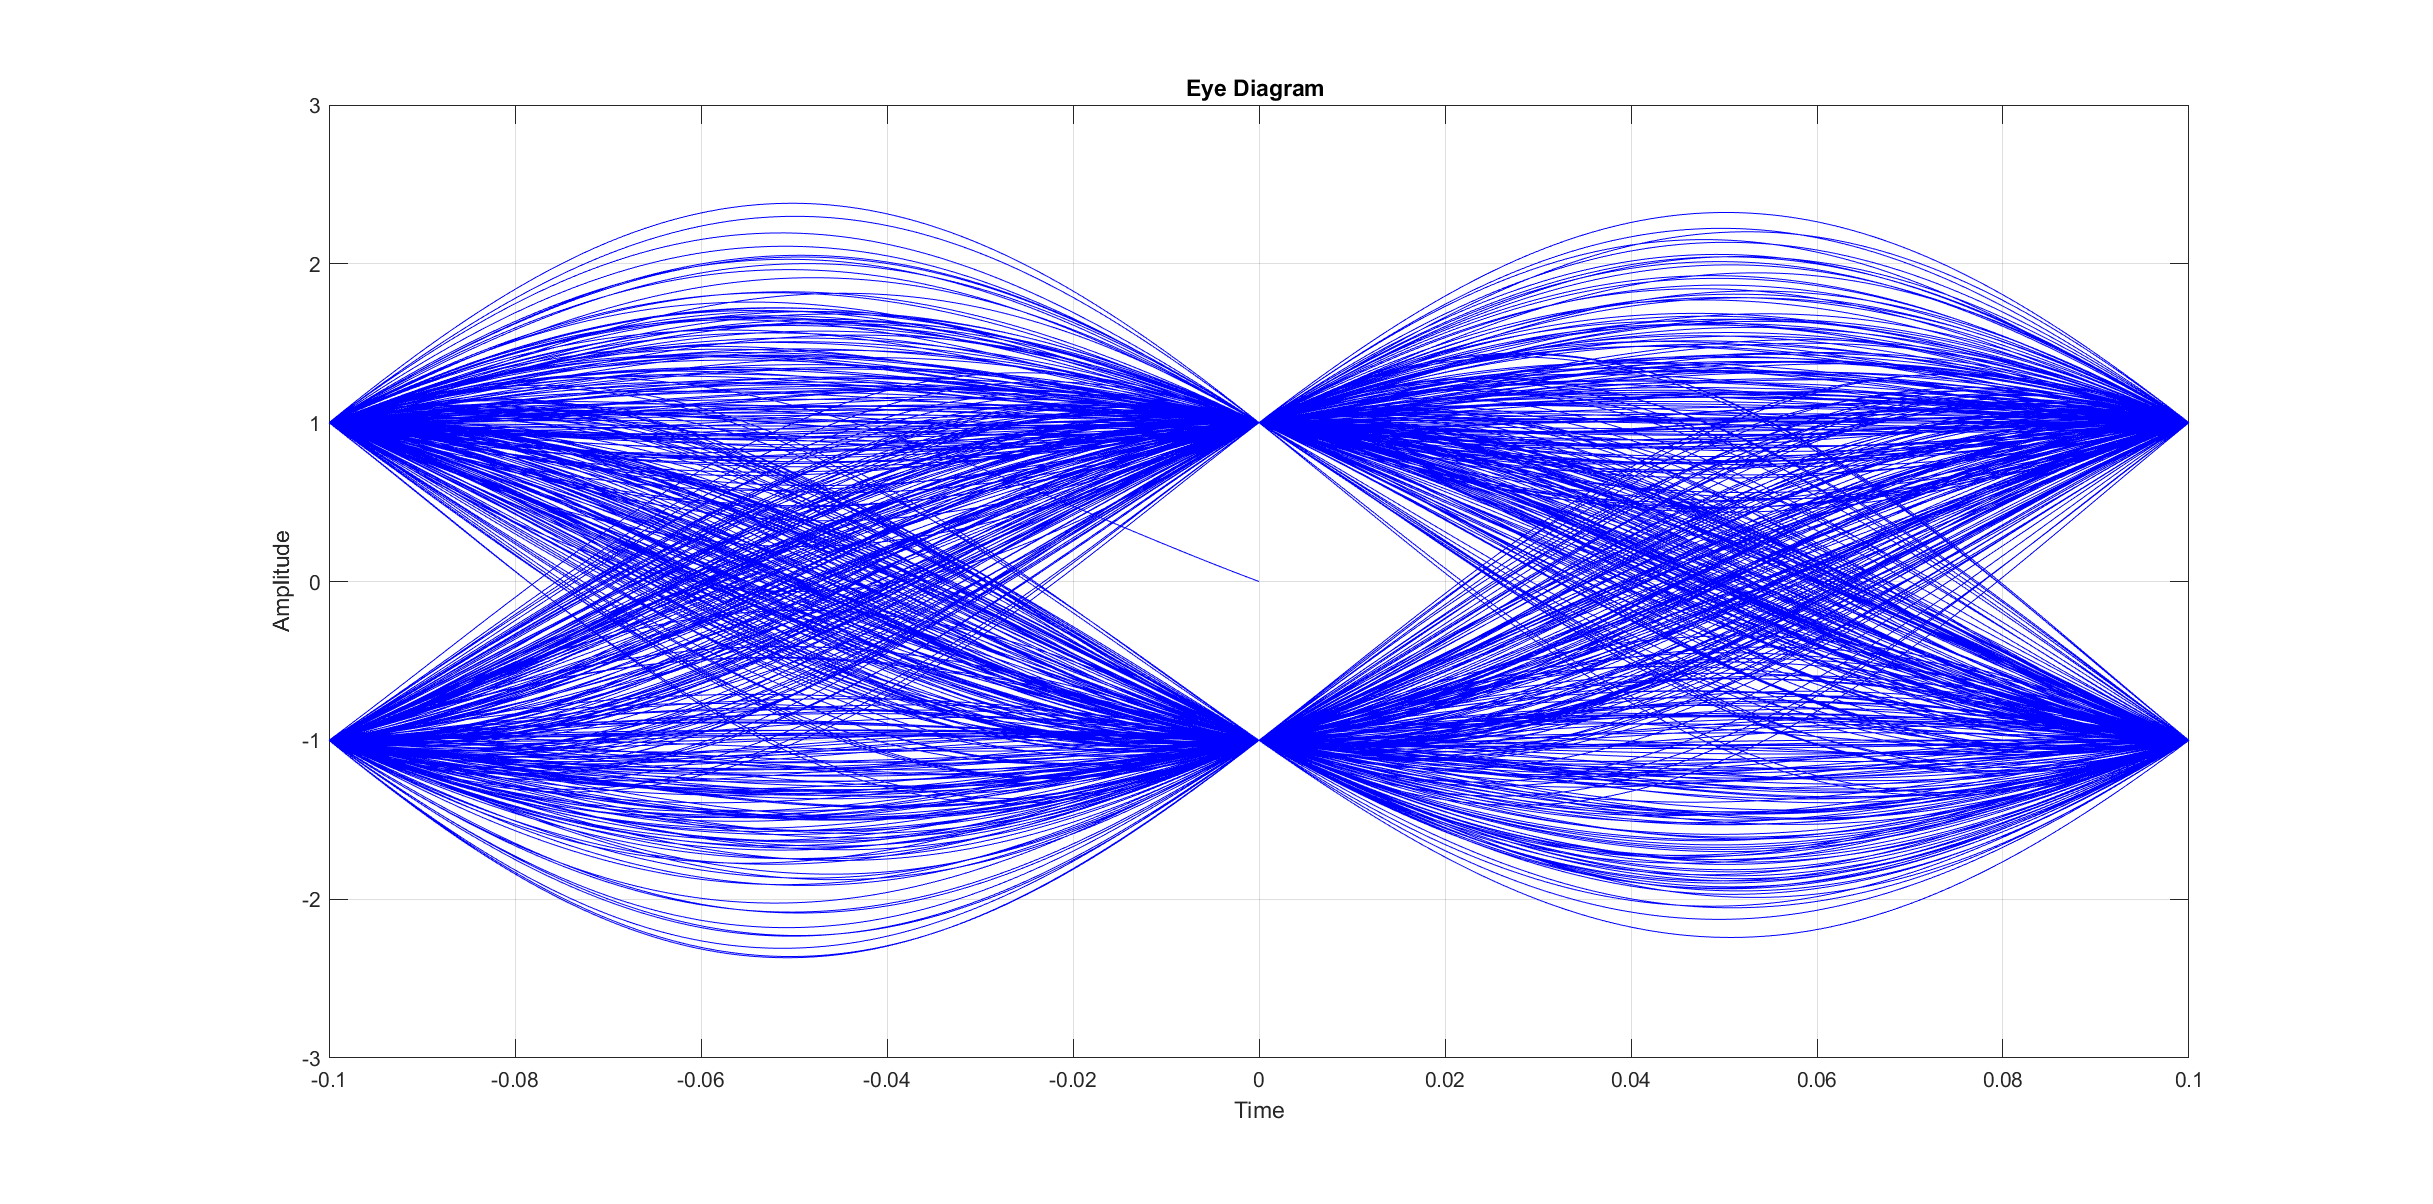
\includegraphics[scale=0.4]{figures/task15}
	\caption{Eye Diagram of the Transmit Signal obtained by Convolving the Impulse train with the Sinc Pulse}
\end{figure}

\subsection{Raised Cosine with with roll-off factor $\alpha = 0.5$ as the Impulse response}
MATLAB's built-in {\tt sinc} and {\tt cosine} functions were used to define the Raised Cosine filters as follows. Where $T_b$ is the separation between successive transmitted pulses.

\[
raised~cosine = sinc(t/T_b)\times \frac{cos(\pi.\alpha.t/T_b)}{ (1 - (2.\alpha.t/Tb)^2 )}
\]

\begin{figure}[H]
	\centering
	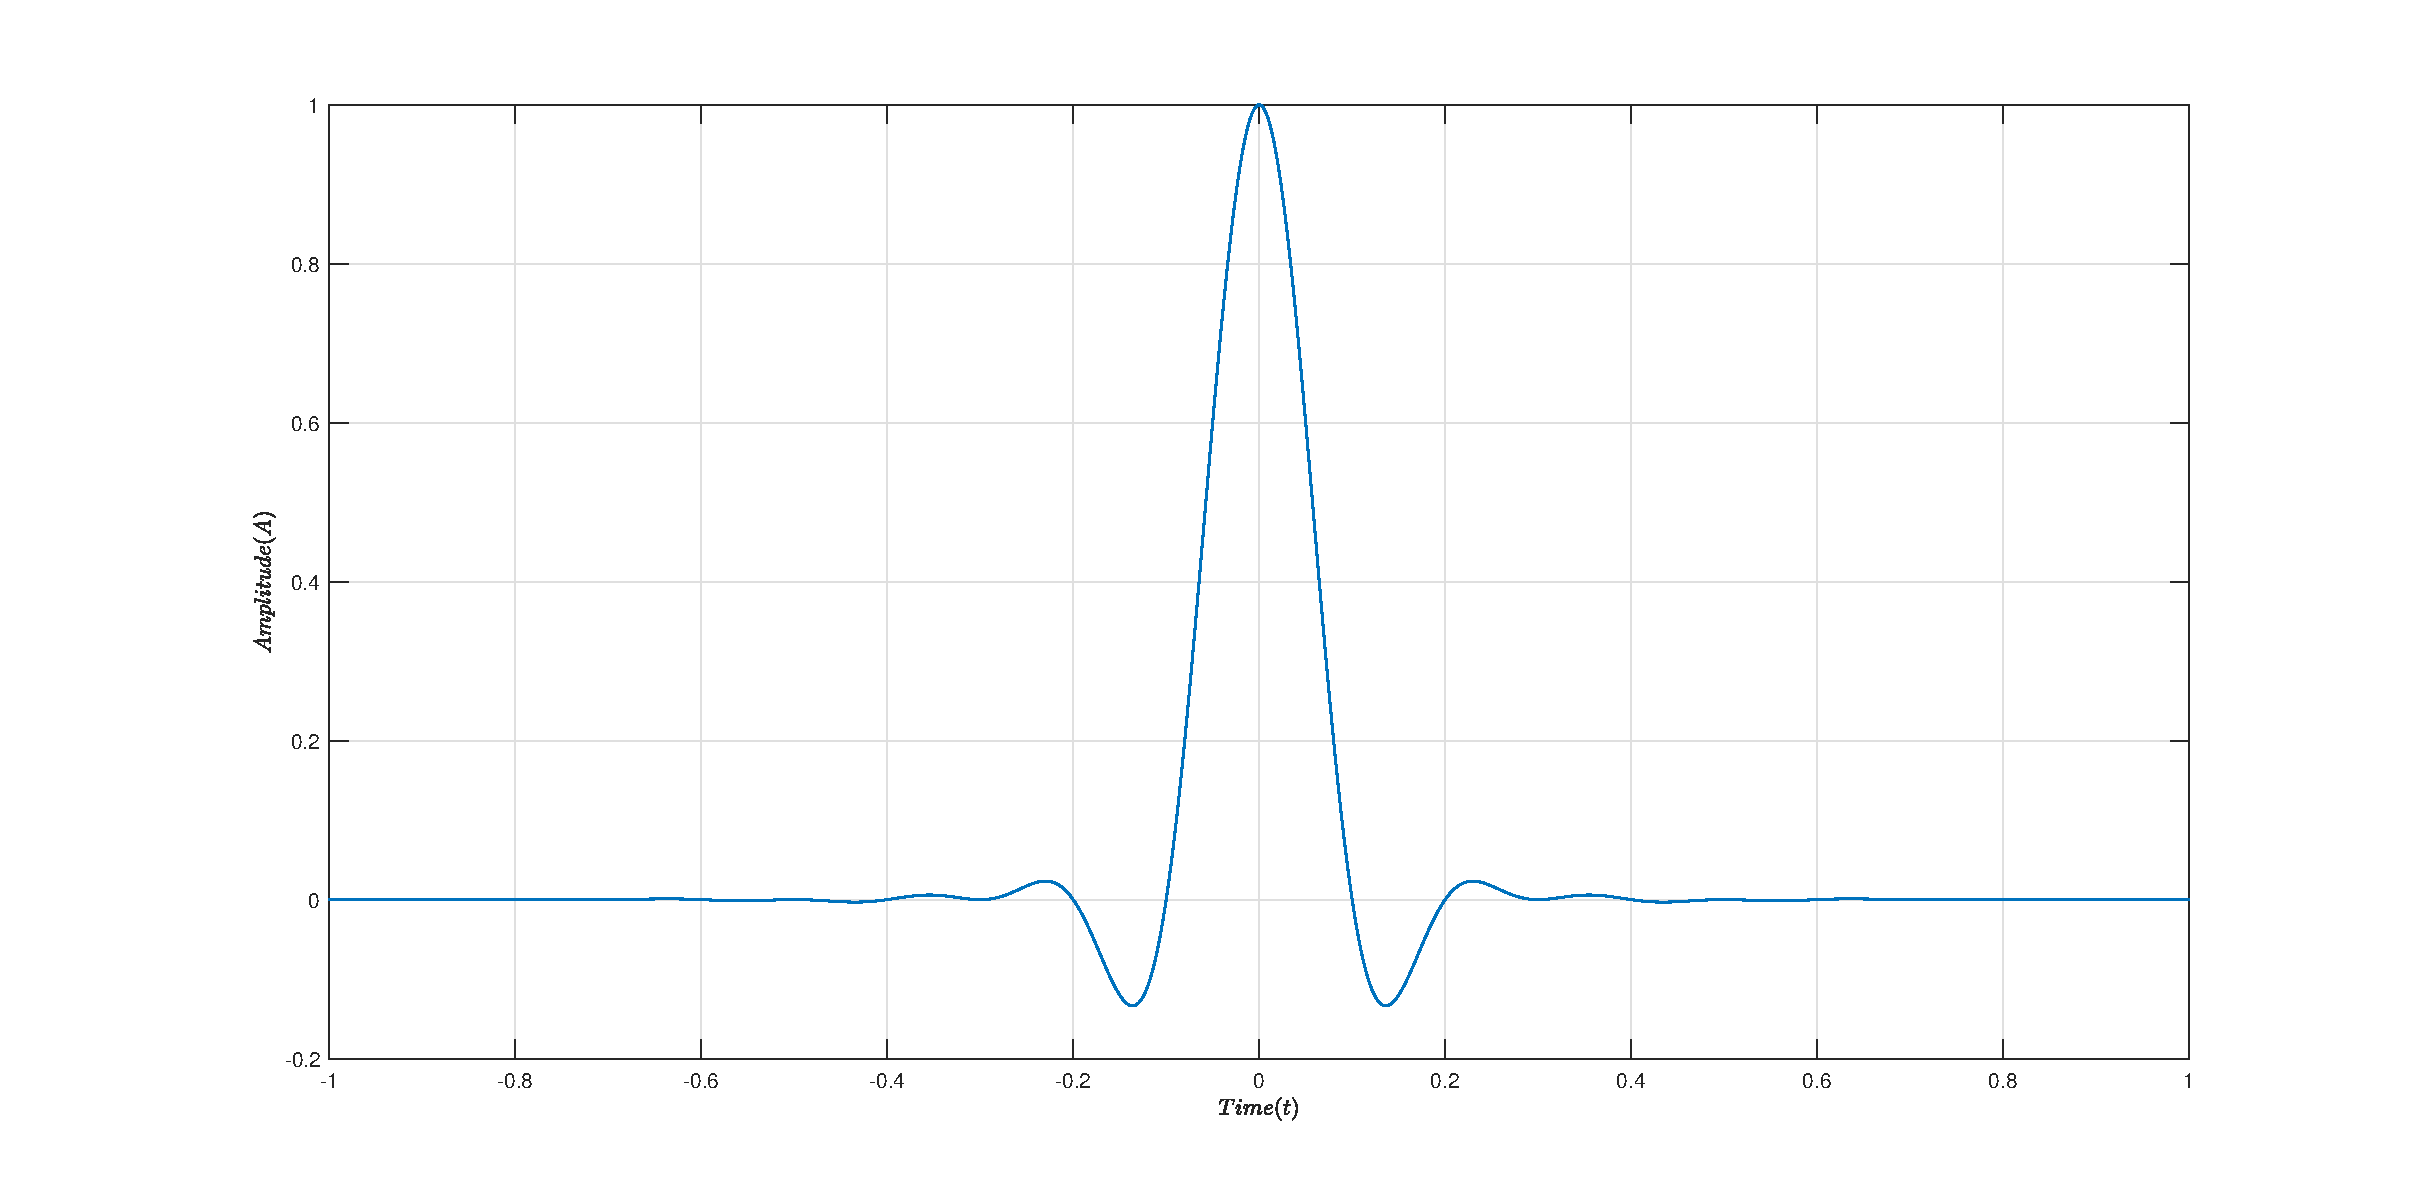
\includegraphics[scale=0.4]{figures/task16}
	\caption{Raised Cosine with with roll-off factor $\alpha = 0.5$ as the Impulse response of the Pulse Shaping Filter}
\end{figure}

\subsection{Convolving the Impulse train with the Raised Cosine with with roll-off factor $\alpha = 0.5$}

\begin{figure}[H]
	\centering
	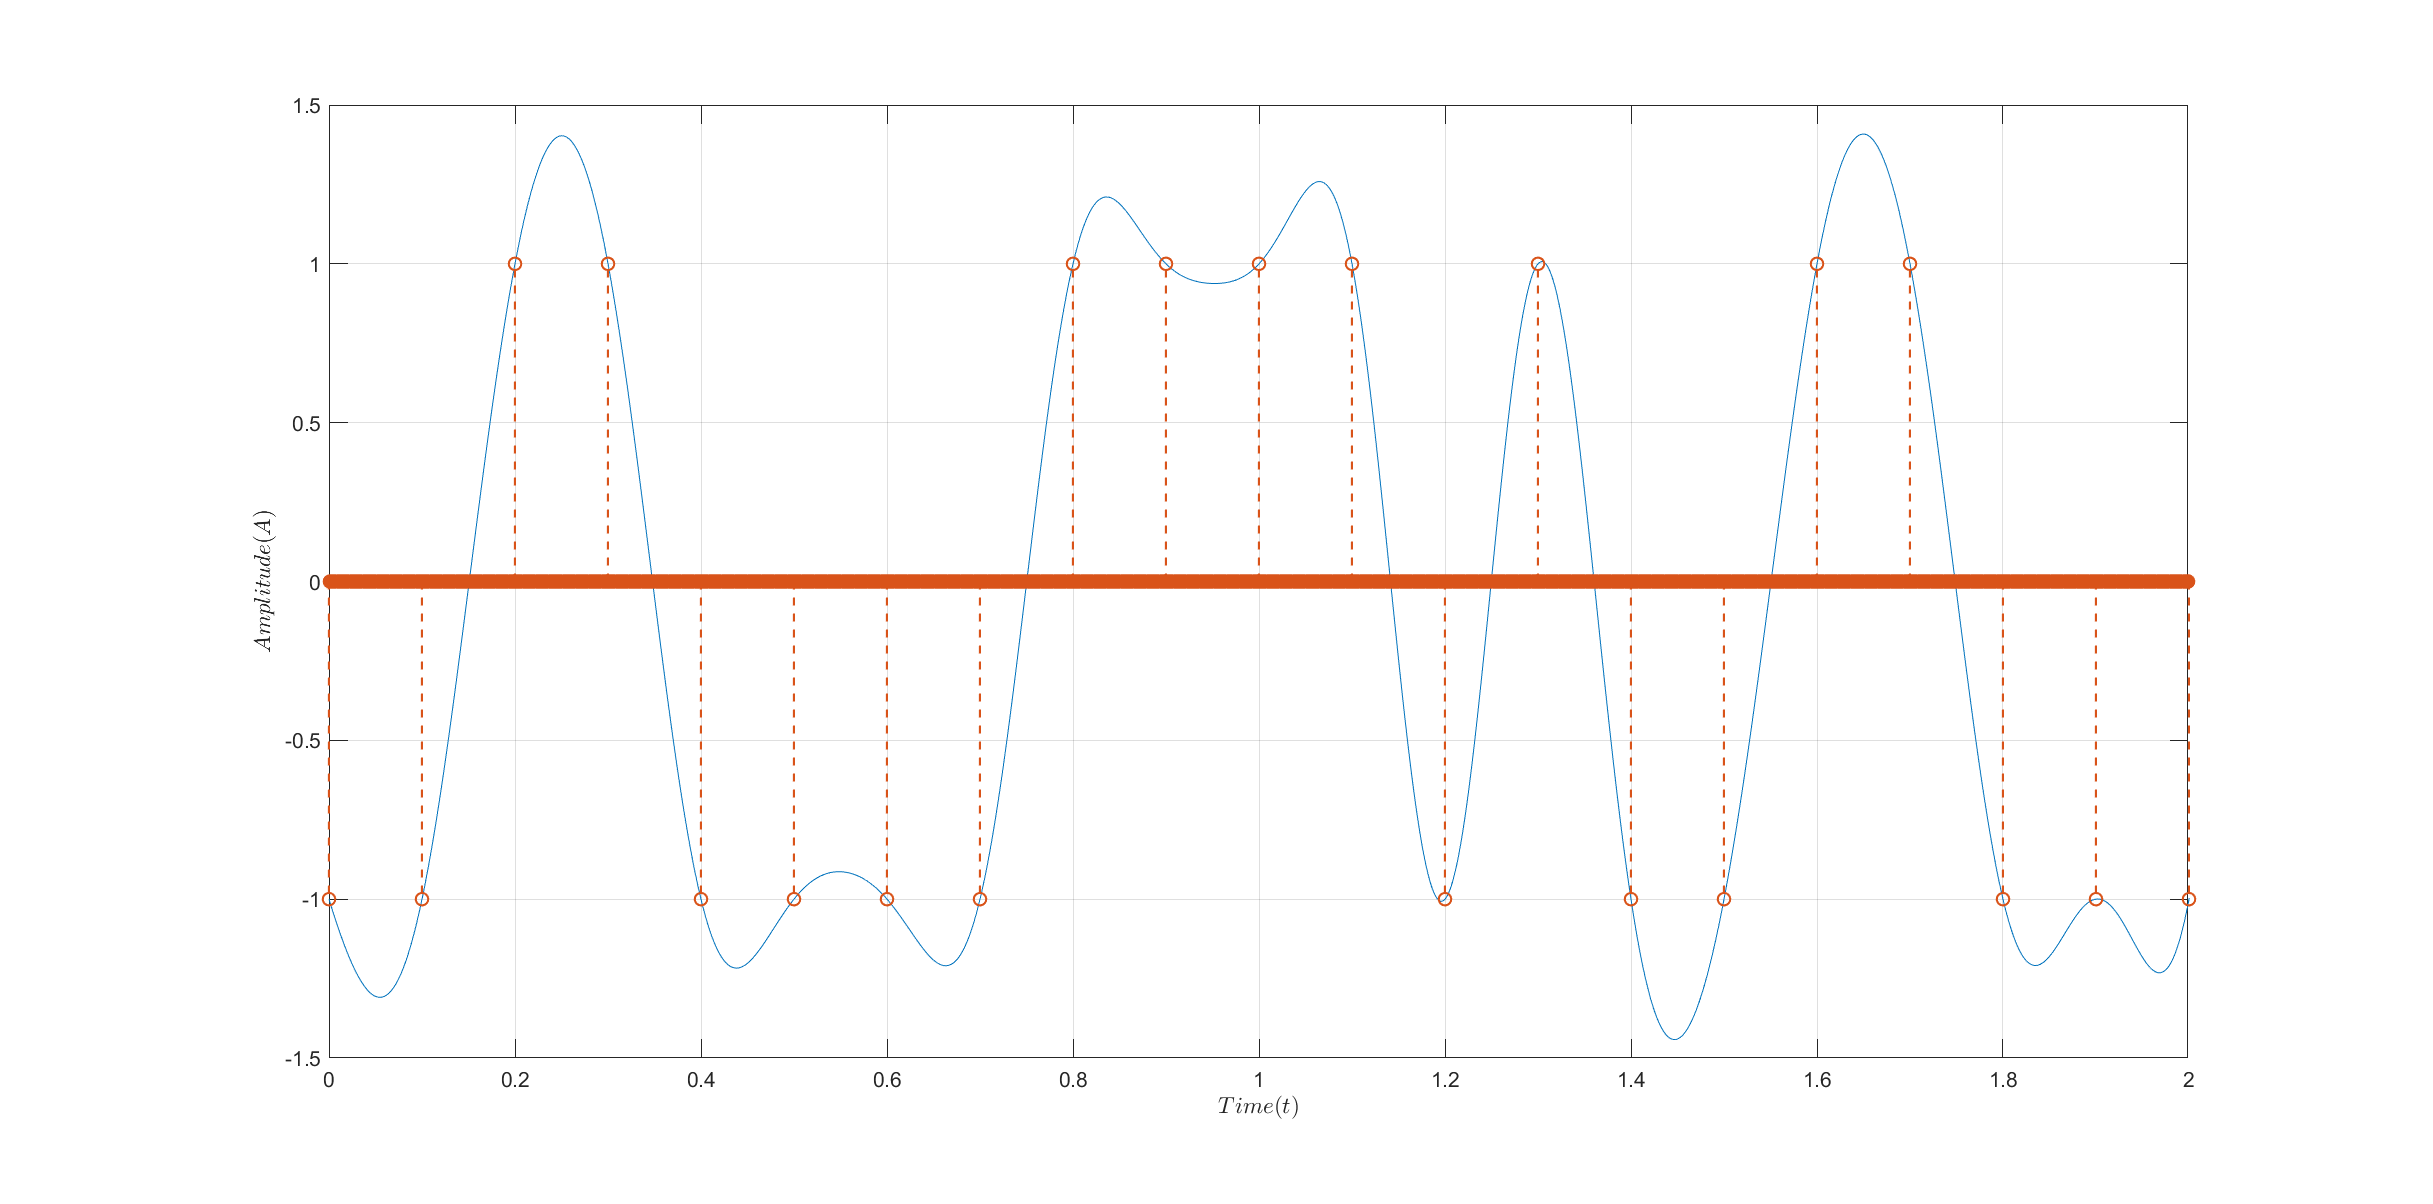
\includegraphics[scale=0.4]{figures/task17}
	\caption{Transmit Signal by Convolving the Impulse train with the Raised Cosine with with roll-off factor $\alpha = 0.5$}
\end{figure}

\subsection{Eye Diagram}

\begin{figure}[H]
	\centering
	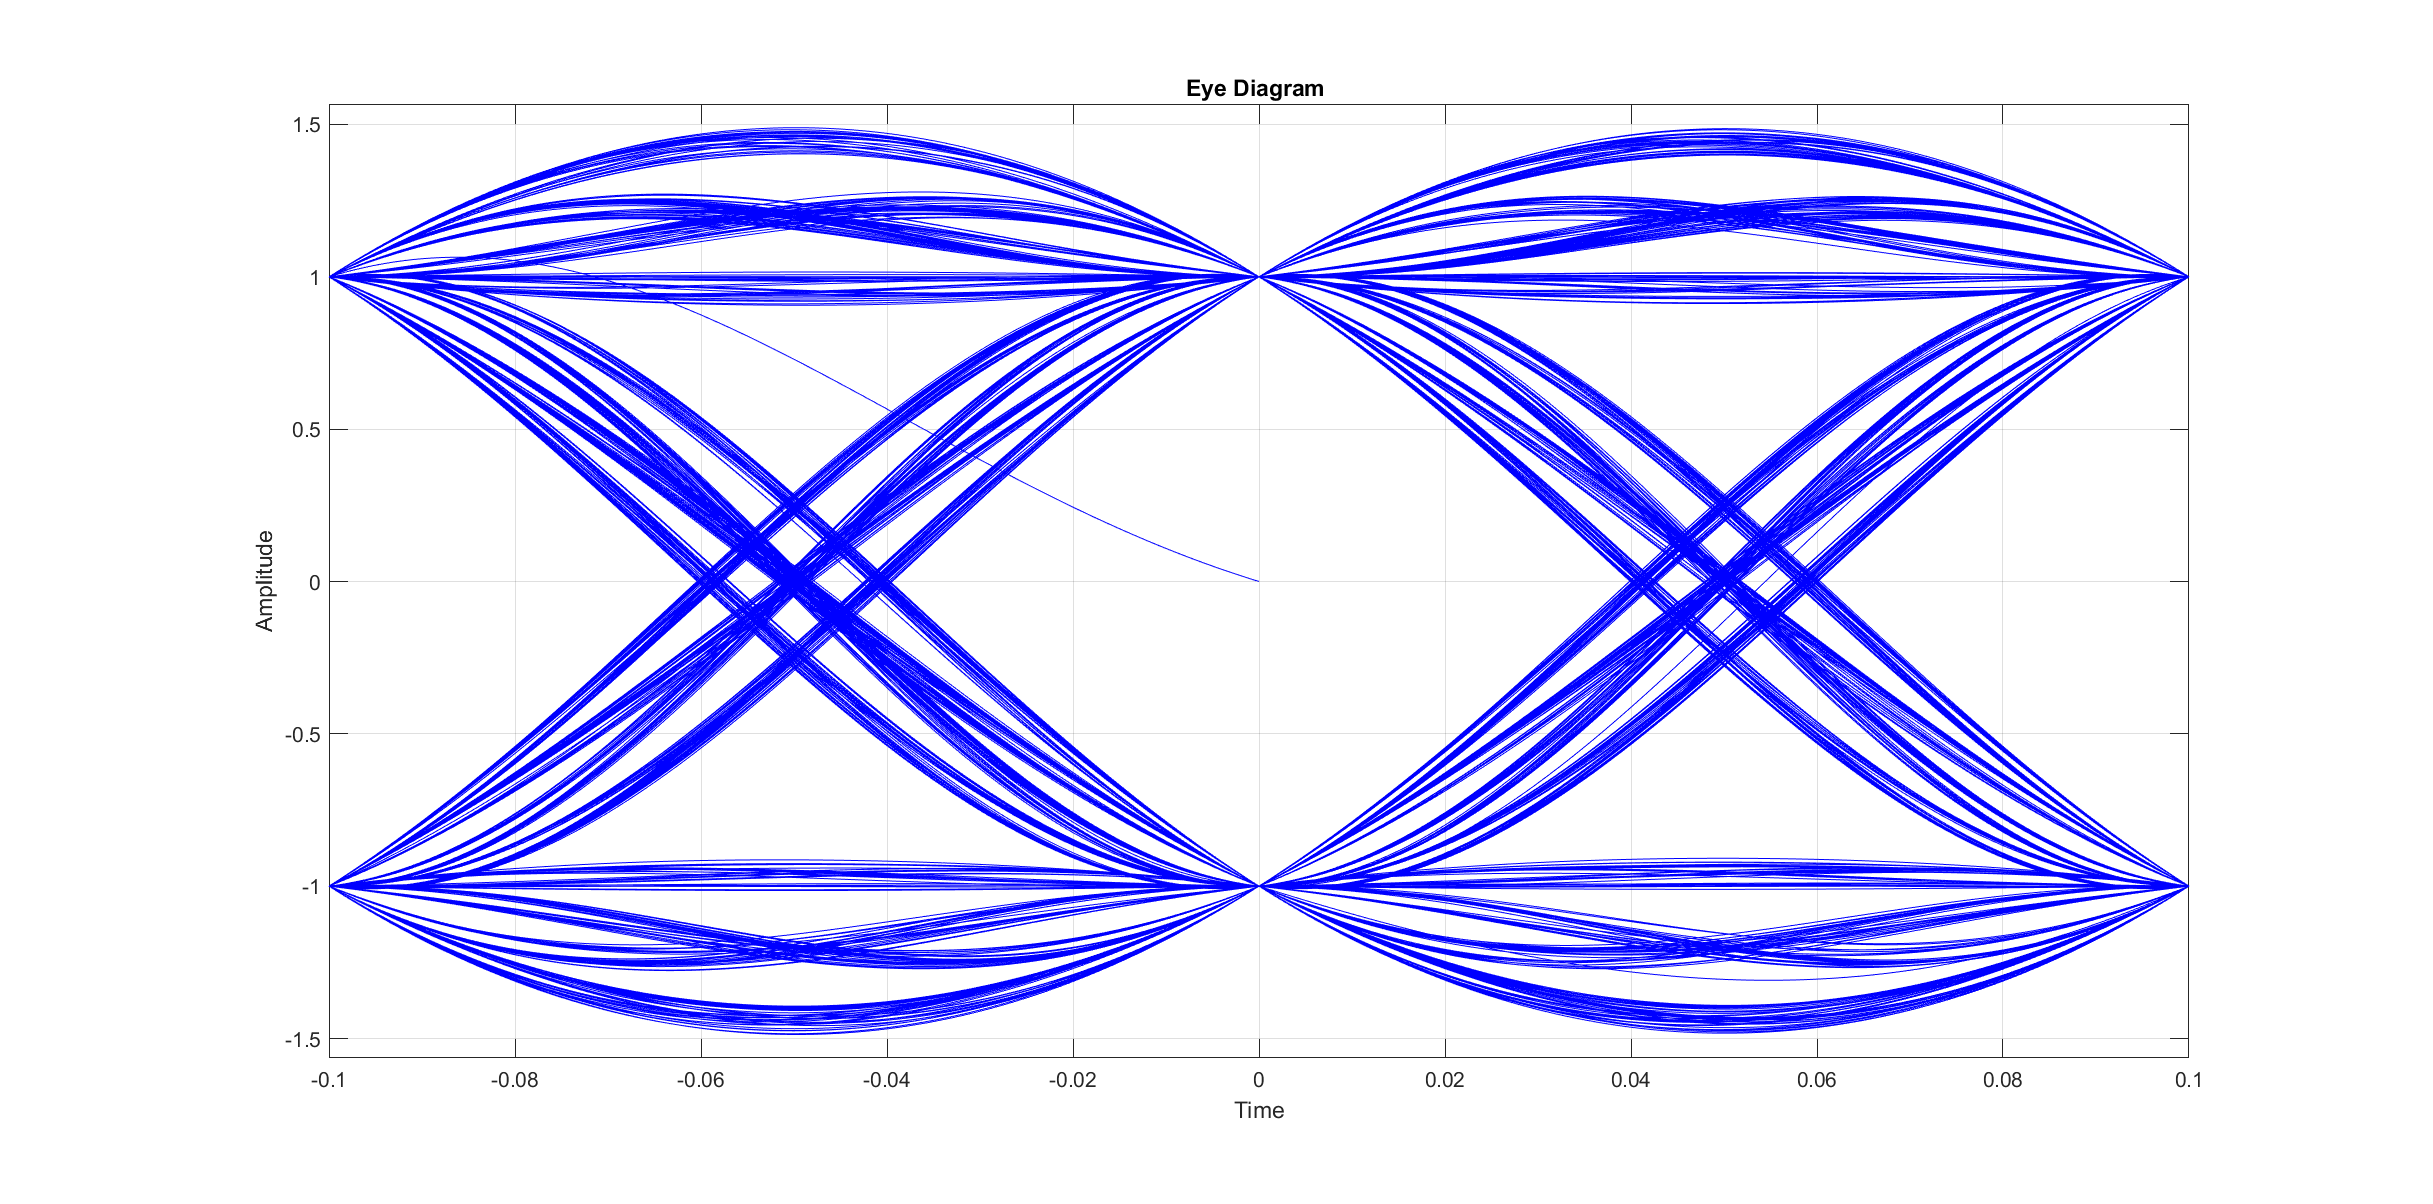
\includegraphics[scale=0.4]{figures/task18}
	\caption{Eye Diagram of the Transmit Signal obtained by Convolving the Impulse train with the Raised Cosine with with roll-off factor $\alpha = 0.5$}
\end{figure}



\subsection{Raised Cosine with with roll-off factor $\alpha = 1$ as the Impulse response}

\begin{figure}[H]
	\centering
	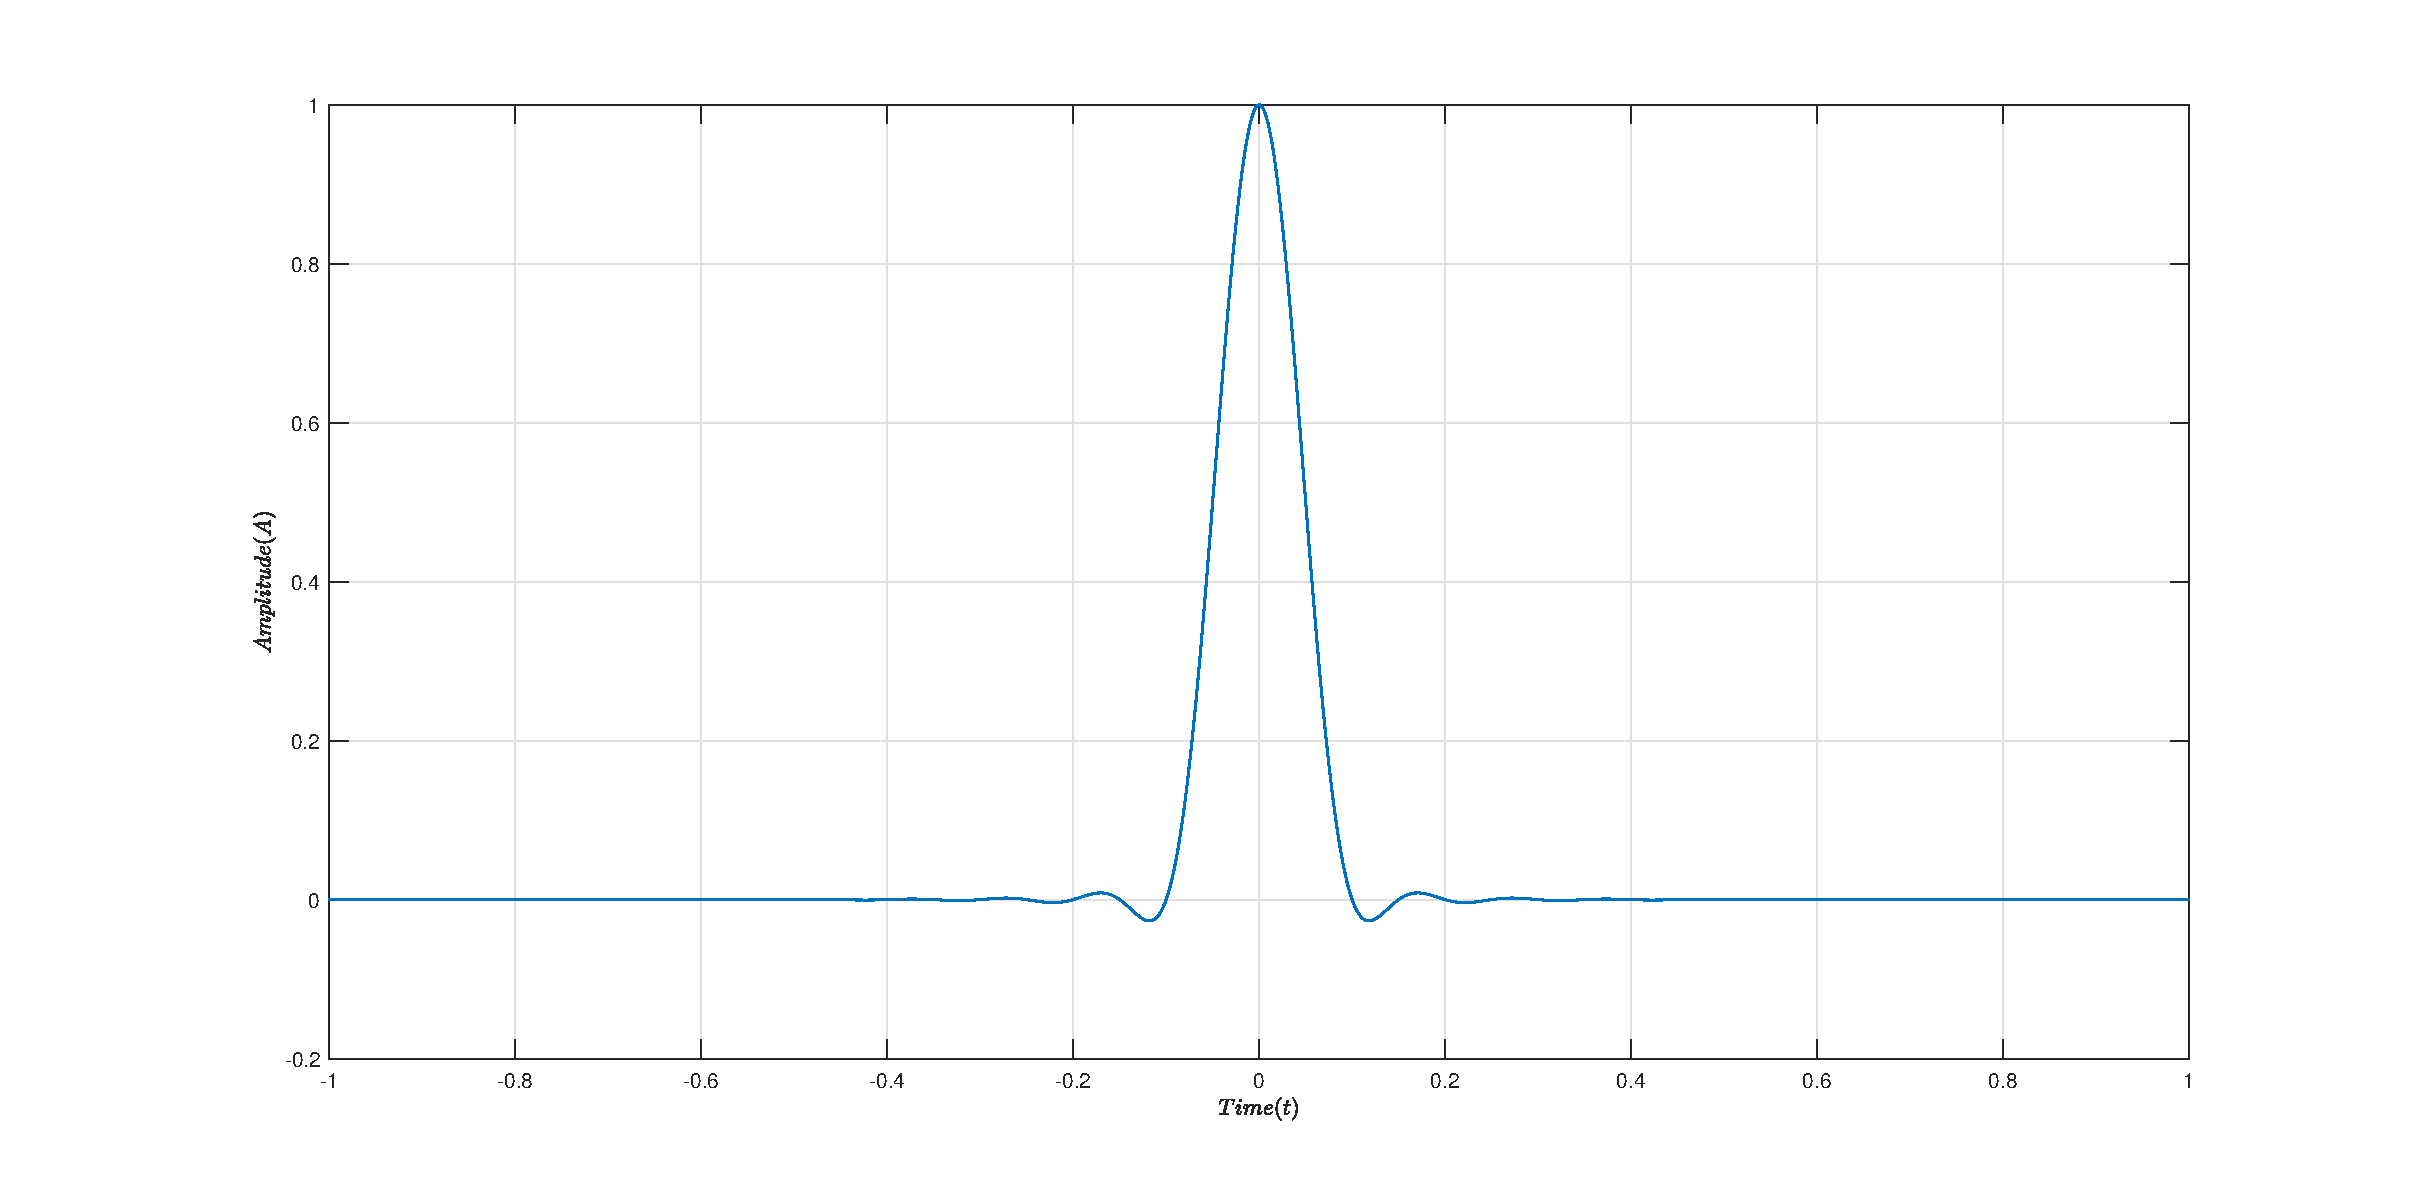
\includegraphics[scale=0.4]{figures/task19}
	\caption{Raised Cosine with with roll-off factor $\alpha = 1$ as the Impulse response of the Pulse Shaping Filter}
\end{figure}

\subsection{Convolving the Impulse train with the Raised Cosine with with roll-off factor $\alpha = 1$}

\begin{figure}[H]
	\centering
	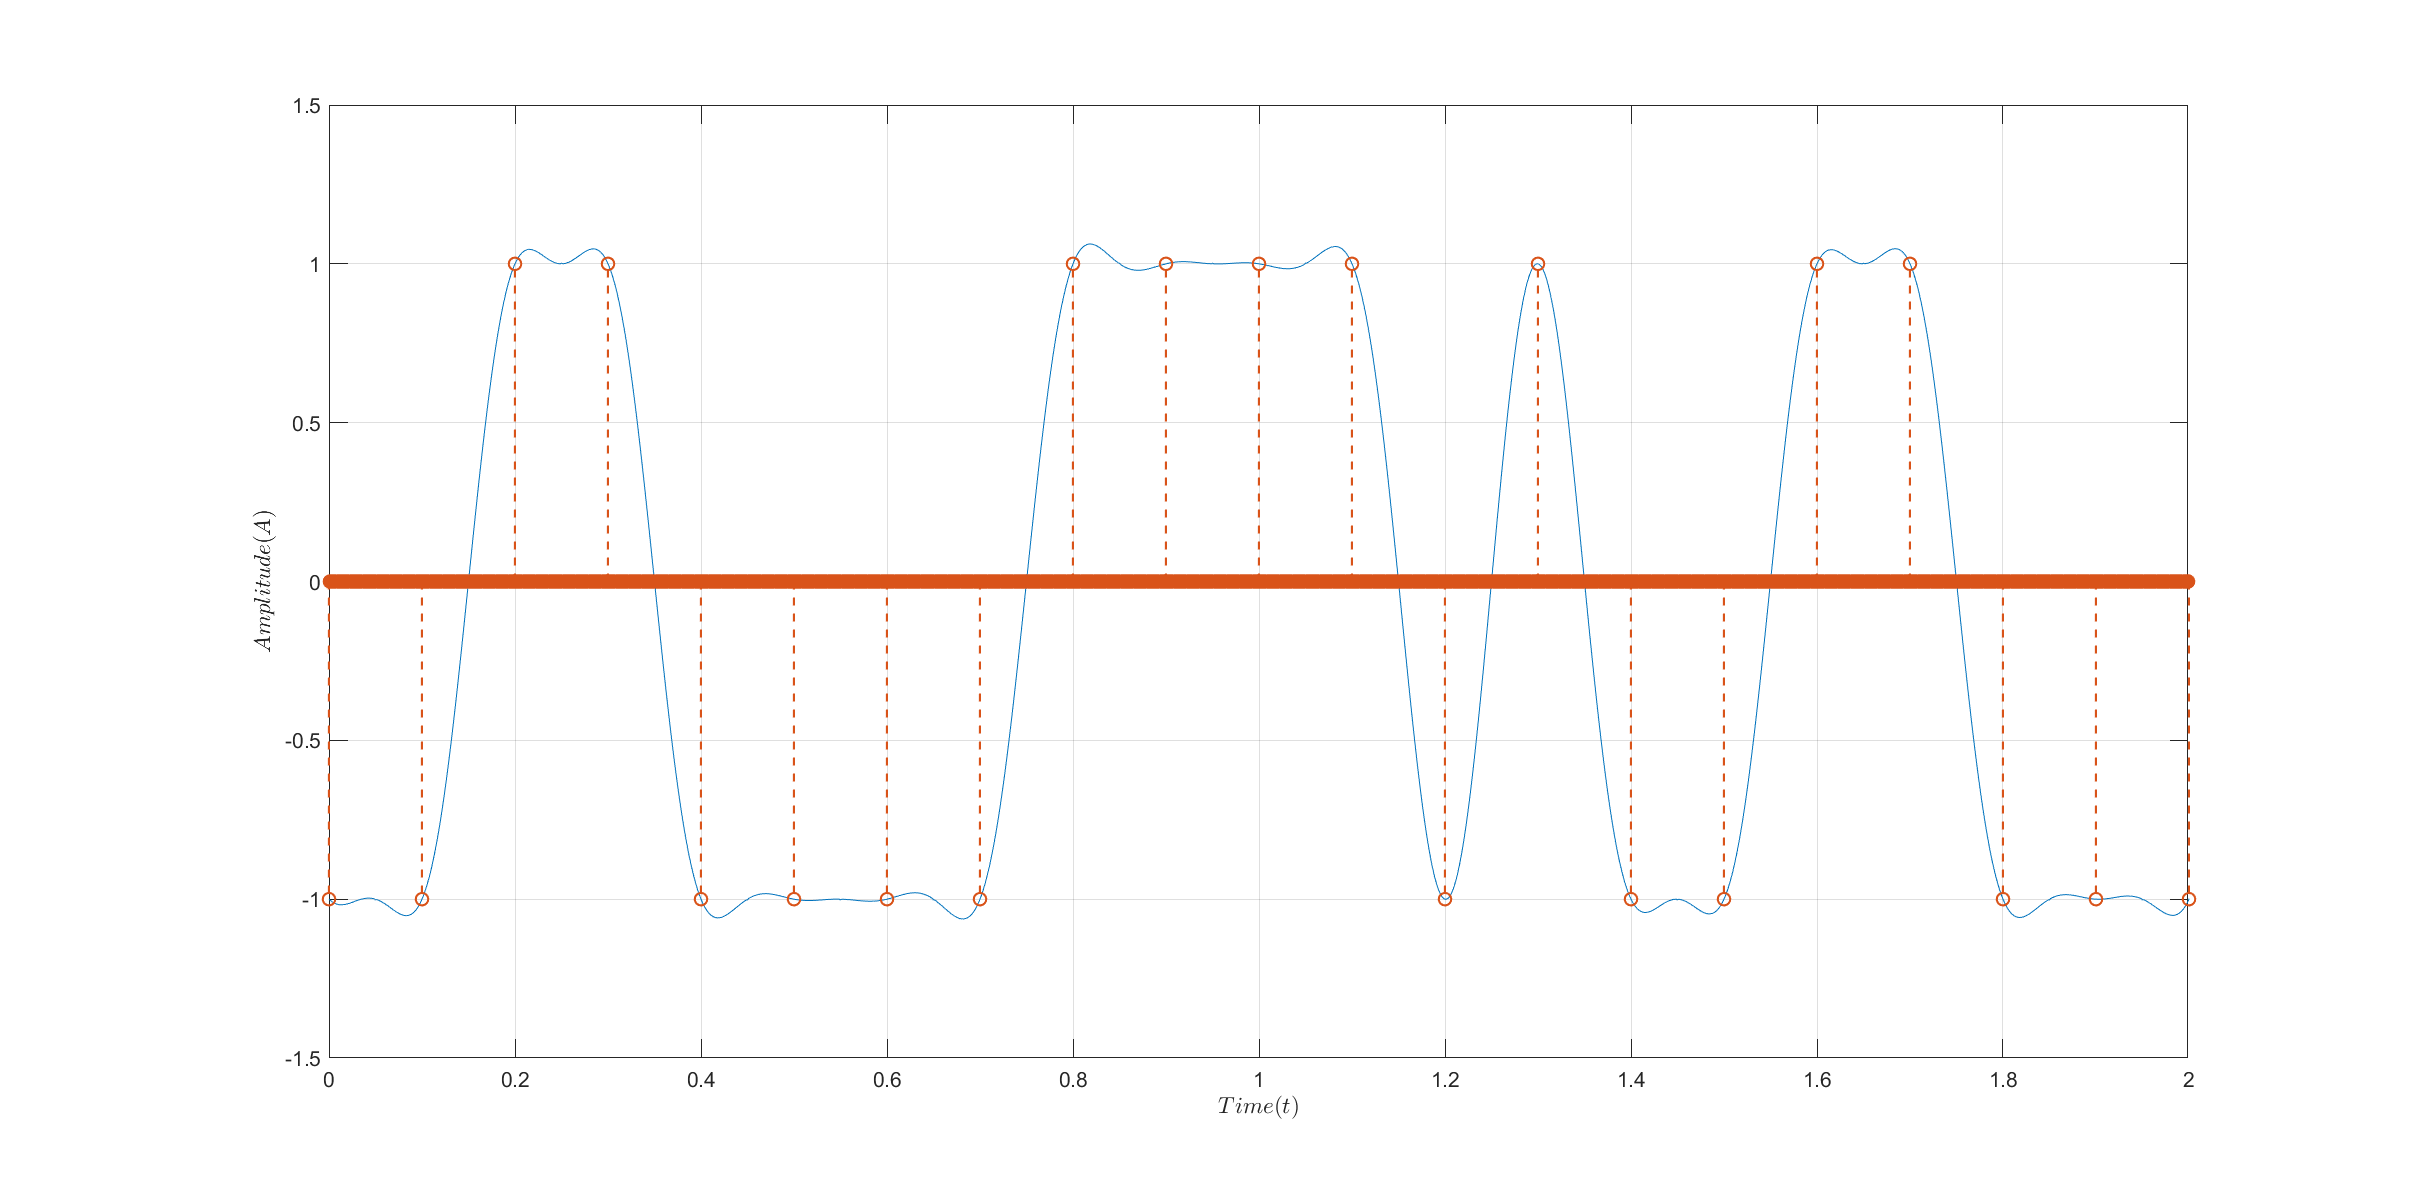
\includegraphics[scale=0.4]{figures/task110}
	\caption{Transmit Signal by Convolving the Impulse train with the Raised Cosine with with roll-off factor $\alpha = 1$}
\end{figure}

\subsection{Eye Diagram}

\begin{figure}[H]
	\centering
	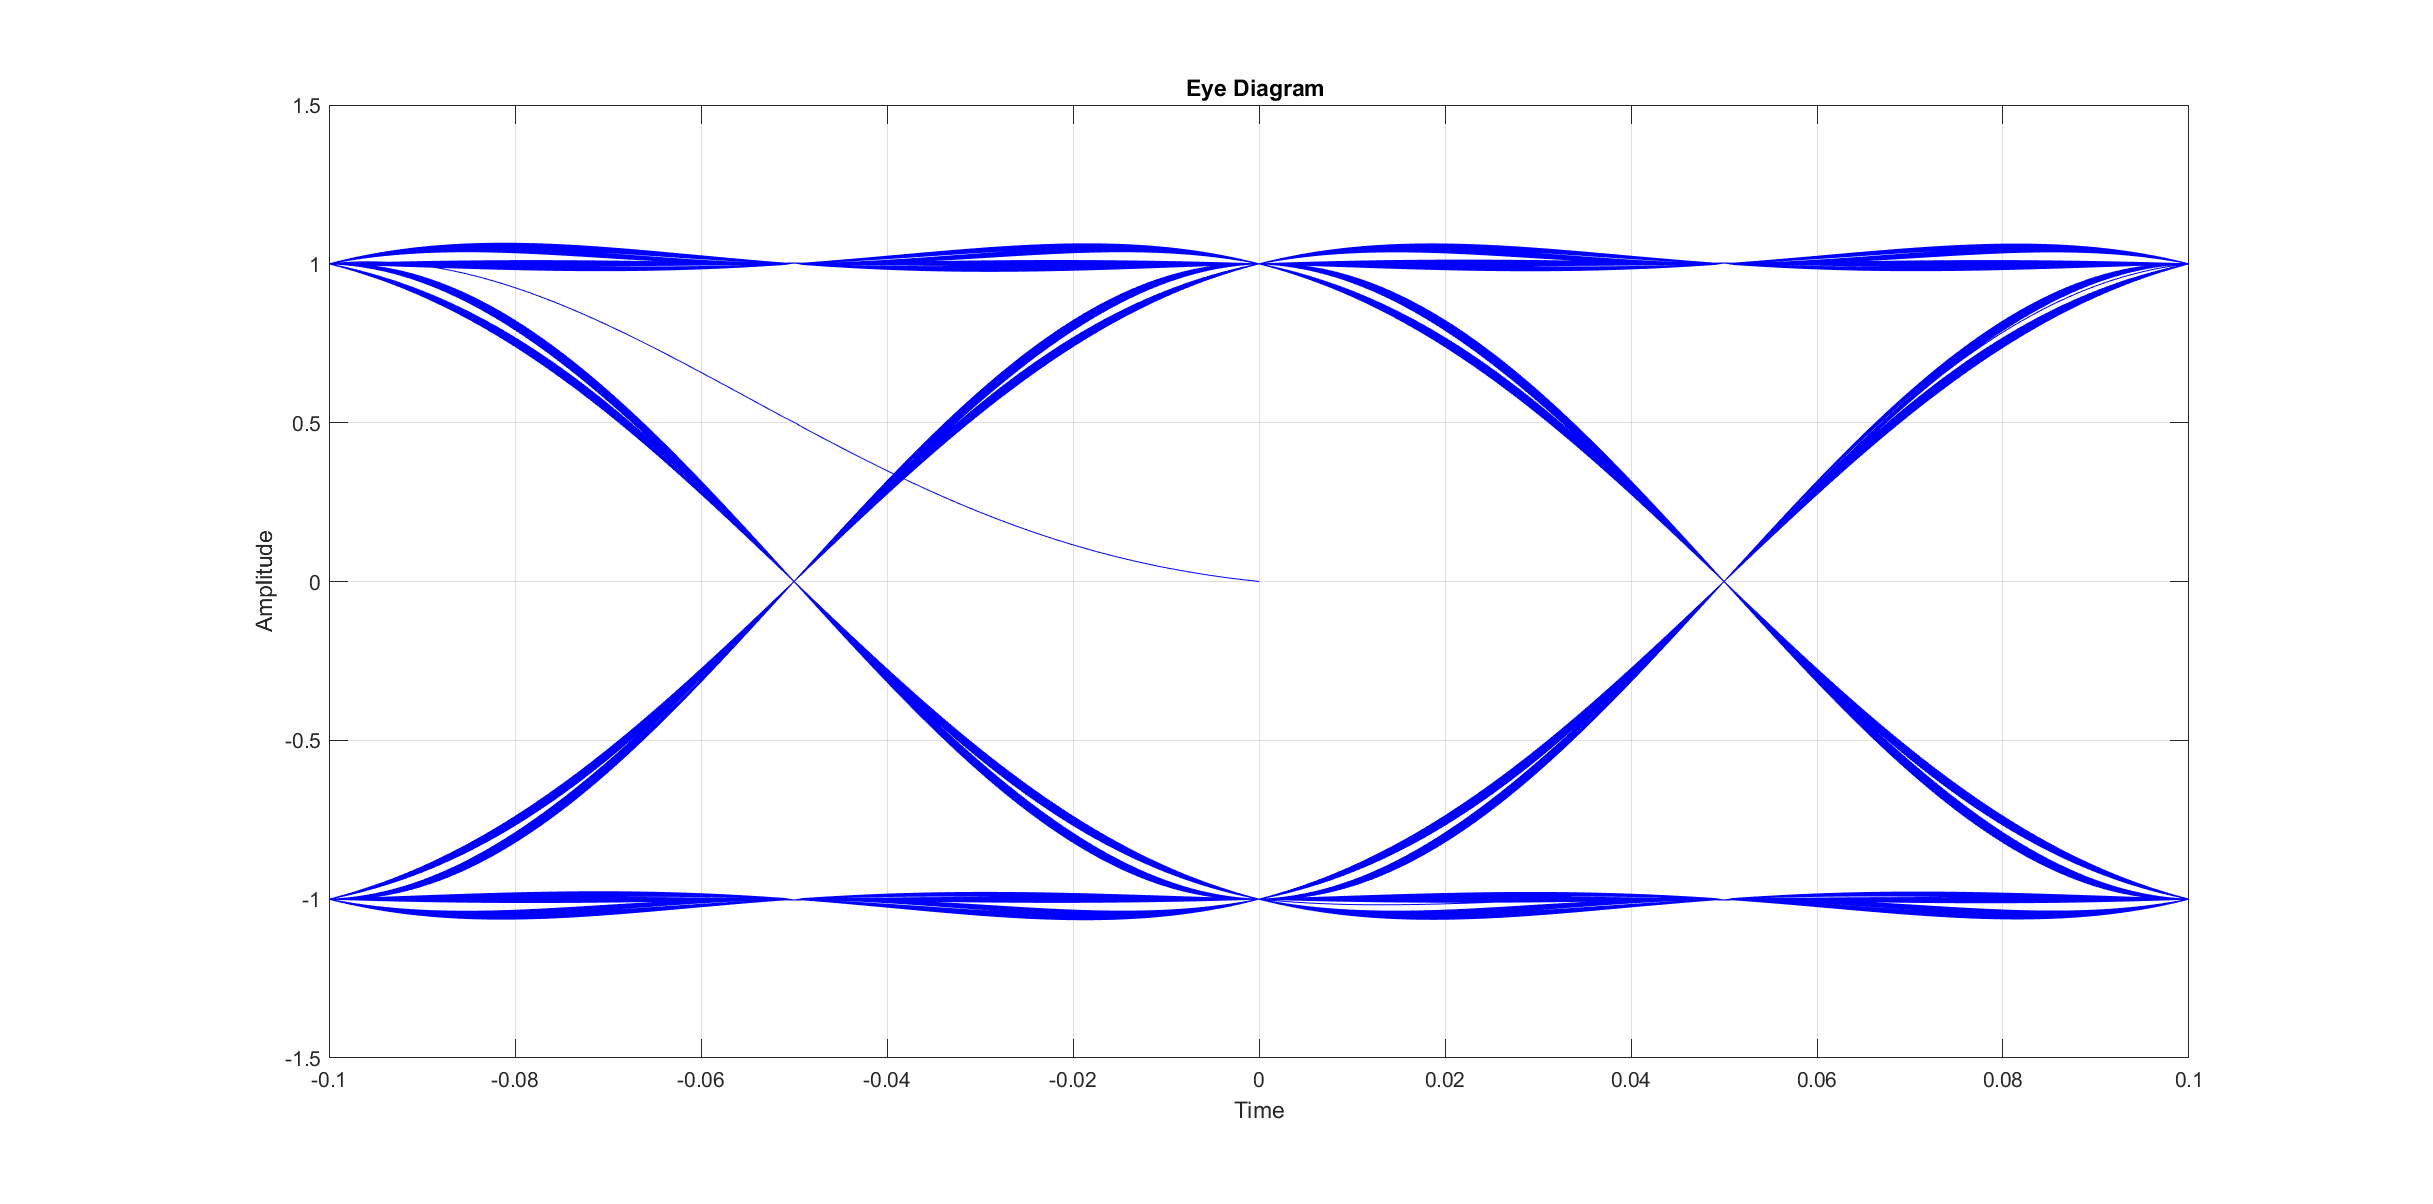
\includegraphics[scale=0.4]{figures/task111}
	\caption{Eye Diagram of the Transmit Signal obtained by Convolving the Impulse train with the Raised Cosine with with roll-off factor $\alpha = 1$}
\end{figure}
\vfill
\subsection{Robustness of the system with respect to noise, sampling time and synchronization errors}

By interpreting the eye diagrams of the above three systems several conclusions can be made on the robustness of those systems.

\begin{itemize}
	\item \textbf{Optimum Sampling Instant at maximum eye opening}: In all the three systems analyzed above , the margin of noise at the optimum sampling instance remain the same under the AWGN free environment.
	\item \textbf{Error-Free Sampling Region}: Width of the eye diagram increases when we move from { \tt sinc} filter to the {\tt raised cosine} filter. That width further increases when we increase the roll-off factor of the raised cosine filter. That is the raised cosine pulse shaping filter has the widest error-free sampling region which makes it more robust.
	\item \textbf{Level-Crossings at the corners of the eye}: {\tt sinc} pulse shaping filter has the maximum level crossing regions at the two corners of the eyes. This implies the highest affect from the Inter Symbol Interference (ISI). Therefore the sinc filter has lower robustness when comparing with the other two systems when it comes to ISI. 
	
\end{itemize}



\section{Task 2}
Task 2 is a repetition of the Task 1, but in the presence of additive white Gaussian noise (AWGN). Variance of the noise $N_0/2$ was set such that the Power efficiency $\gamma = E_b/N_0 = 10 ~dB$. Where $E_b$ is the average bit energy and $N_0$ is the noise power spectral density.

\[
\begin{split}
	\gamma~in~dB &= 10.\log_{10}(E_b/N_0)\\
	\gamma/10 &= \log_{10}(E_b/N_0)\\
	10^{\gamma/10} &= E_b/N_0\\
	N_0 &= \frac{E_b}{10^{\gamma/10}}
\end{split}
\]

\[\therefore ~\sigma_{noise}^2 = N_0/2 = \frac{E_b}{2 \times 10^{\gamma/10}}  \]
Assuming the $P(D = 0) = P(D = 1) = 1/2$ as we consider sufficient large amount of bits in the initial bit stream,
\[
E_b = \frac{1}{2} \times \left[ (+A)^2 + (-A)^2 \right]
 = \frac{1}{2} \times \left[ (+1)^2 + (-1)^2 \right]
 = 1
\]
\pagebreak
\subsection{Affect of AWGN, when using the Sinc function as the Impulse response}

\begin{figure}[H]
	\centering
	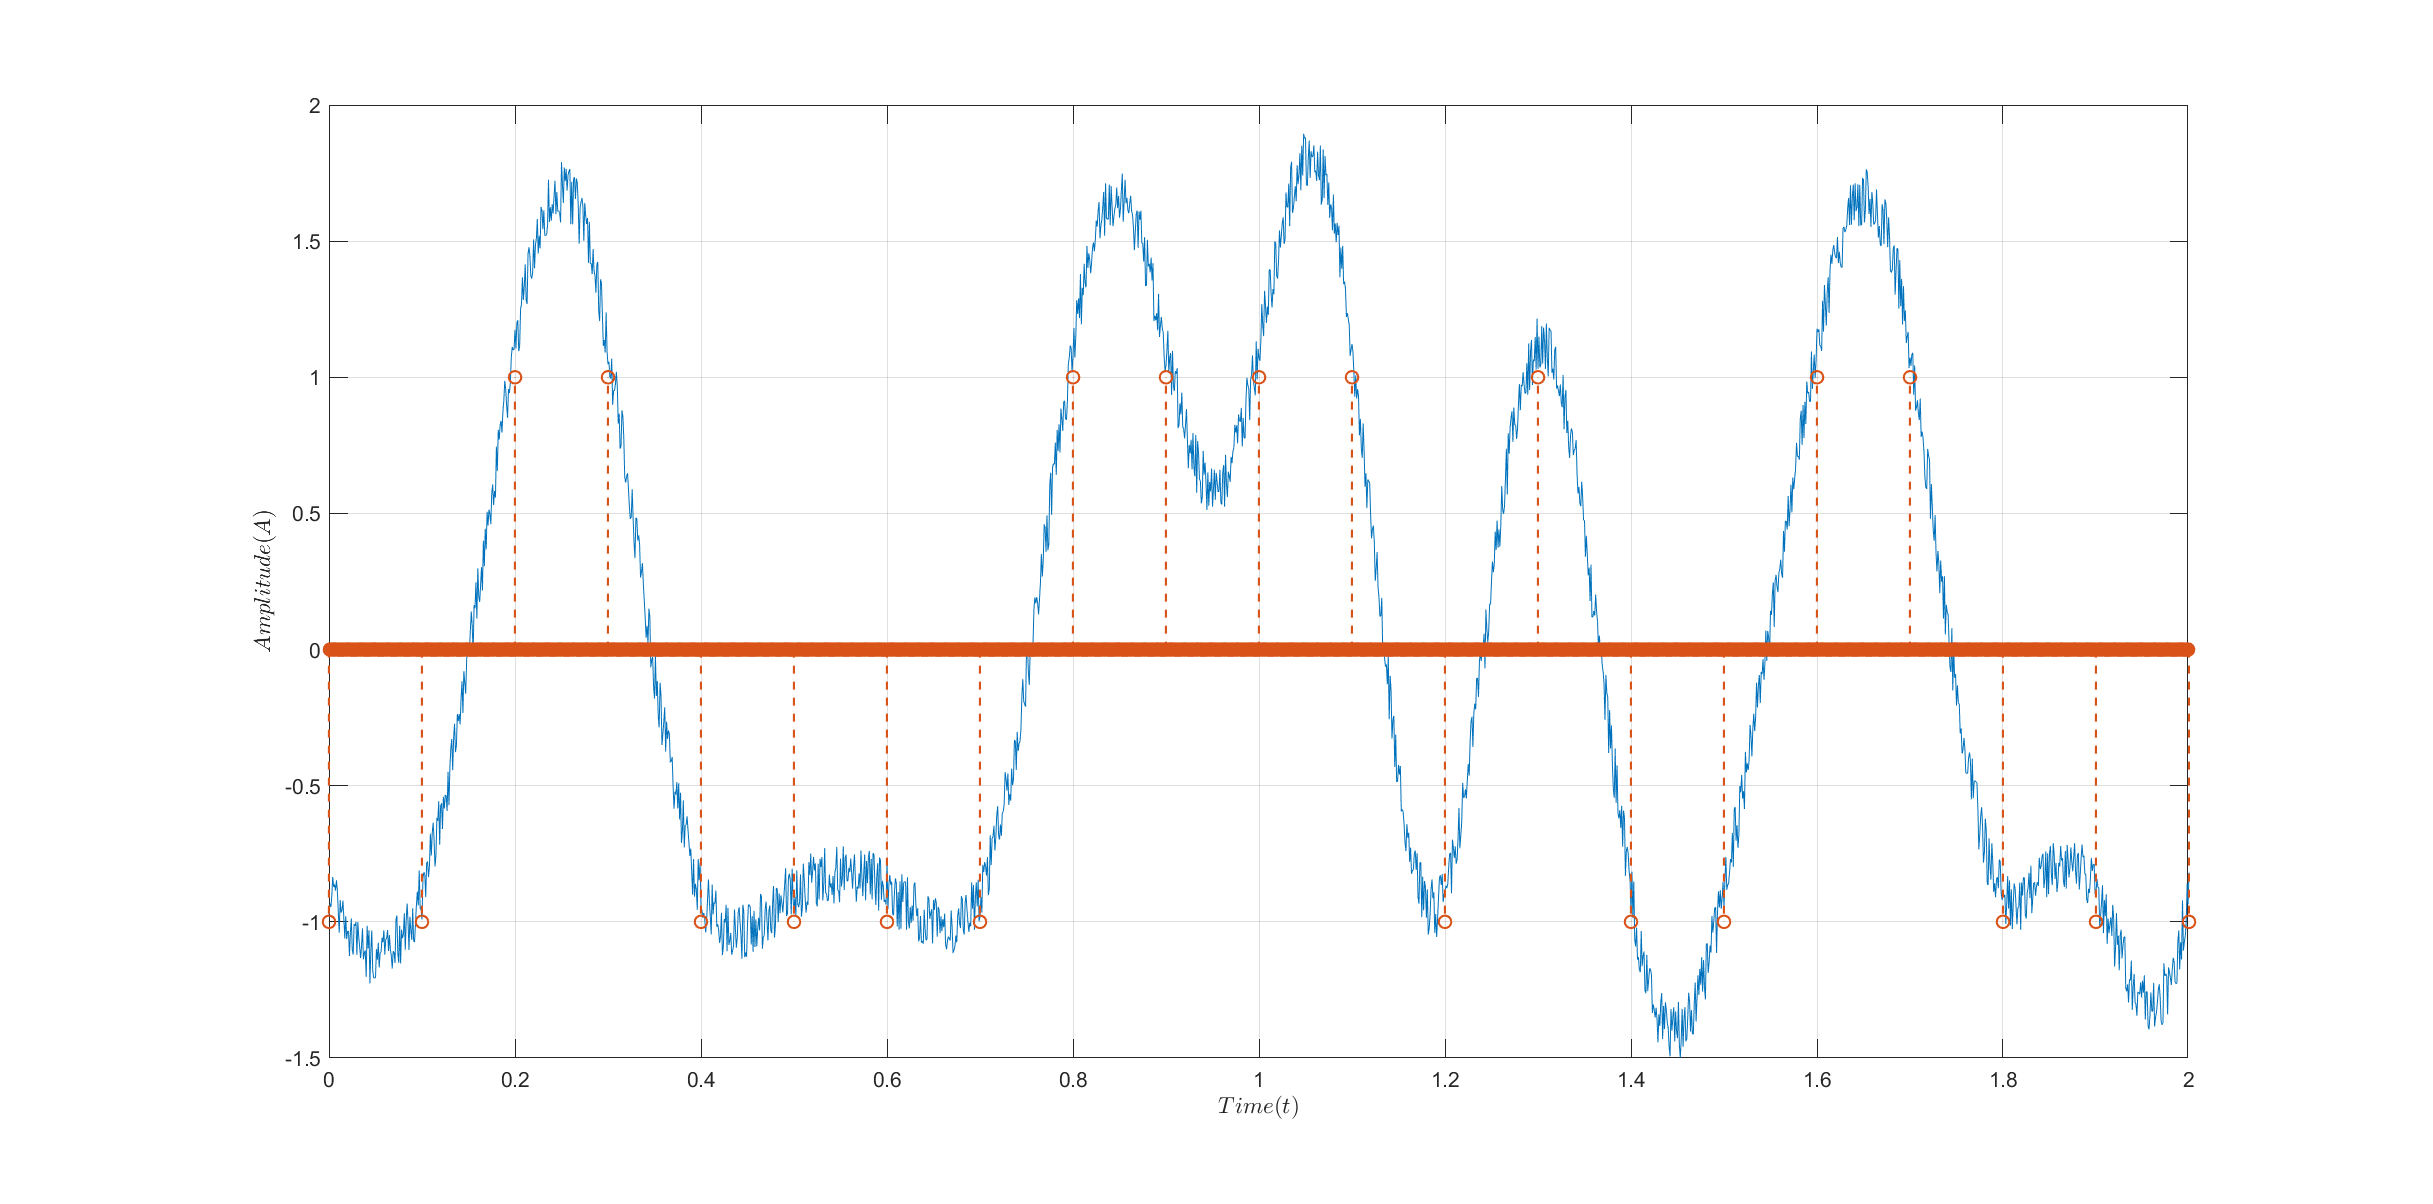
\includegraphics[scale=0.4]{figures/task21}
	\caption{Transmit Signal}
\end{figure}

\begin{figure}[H]
	\centering
	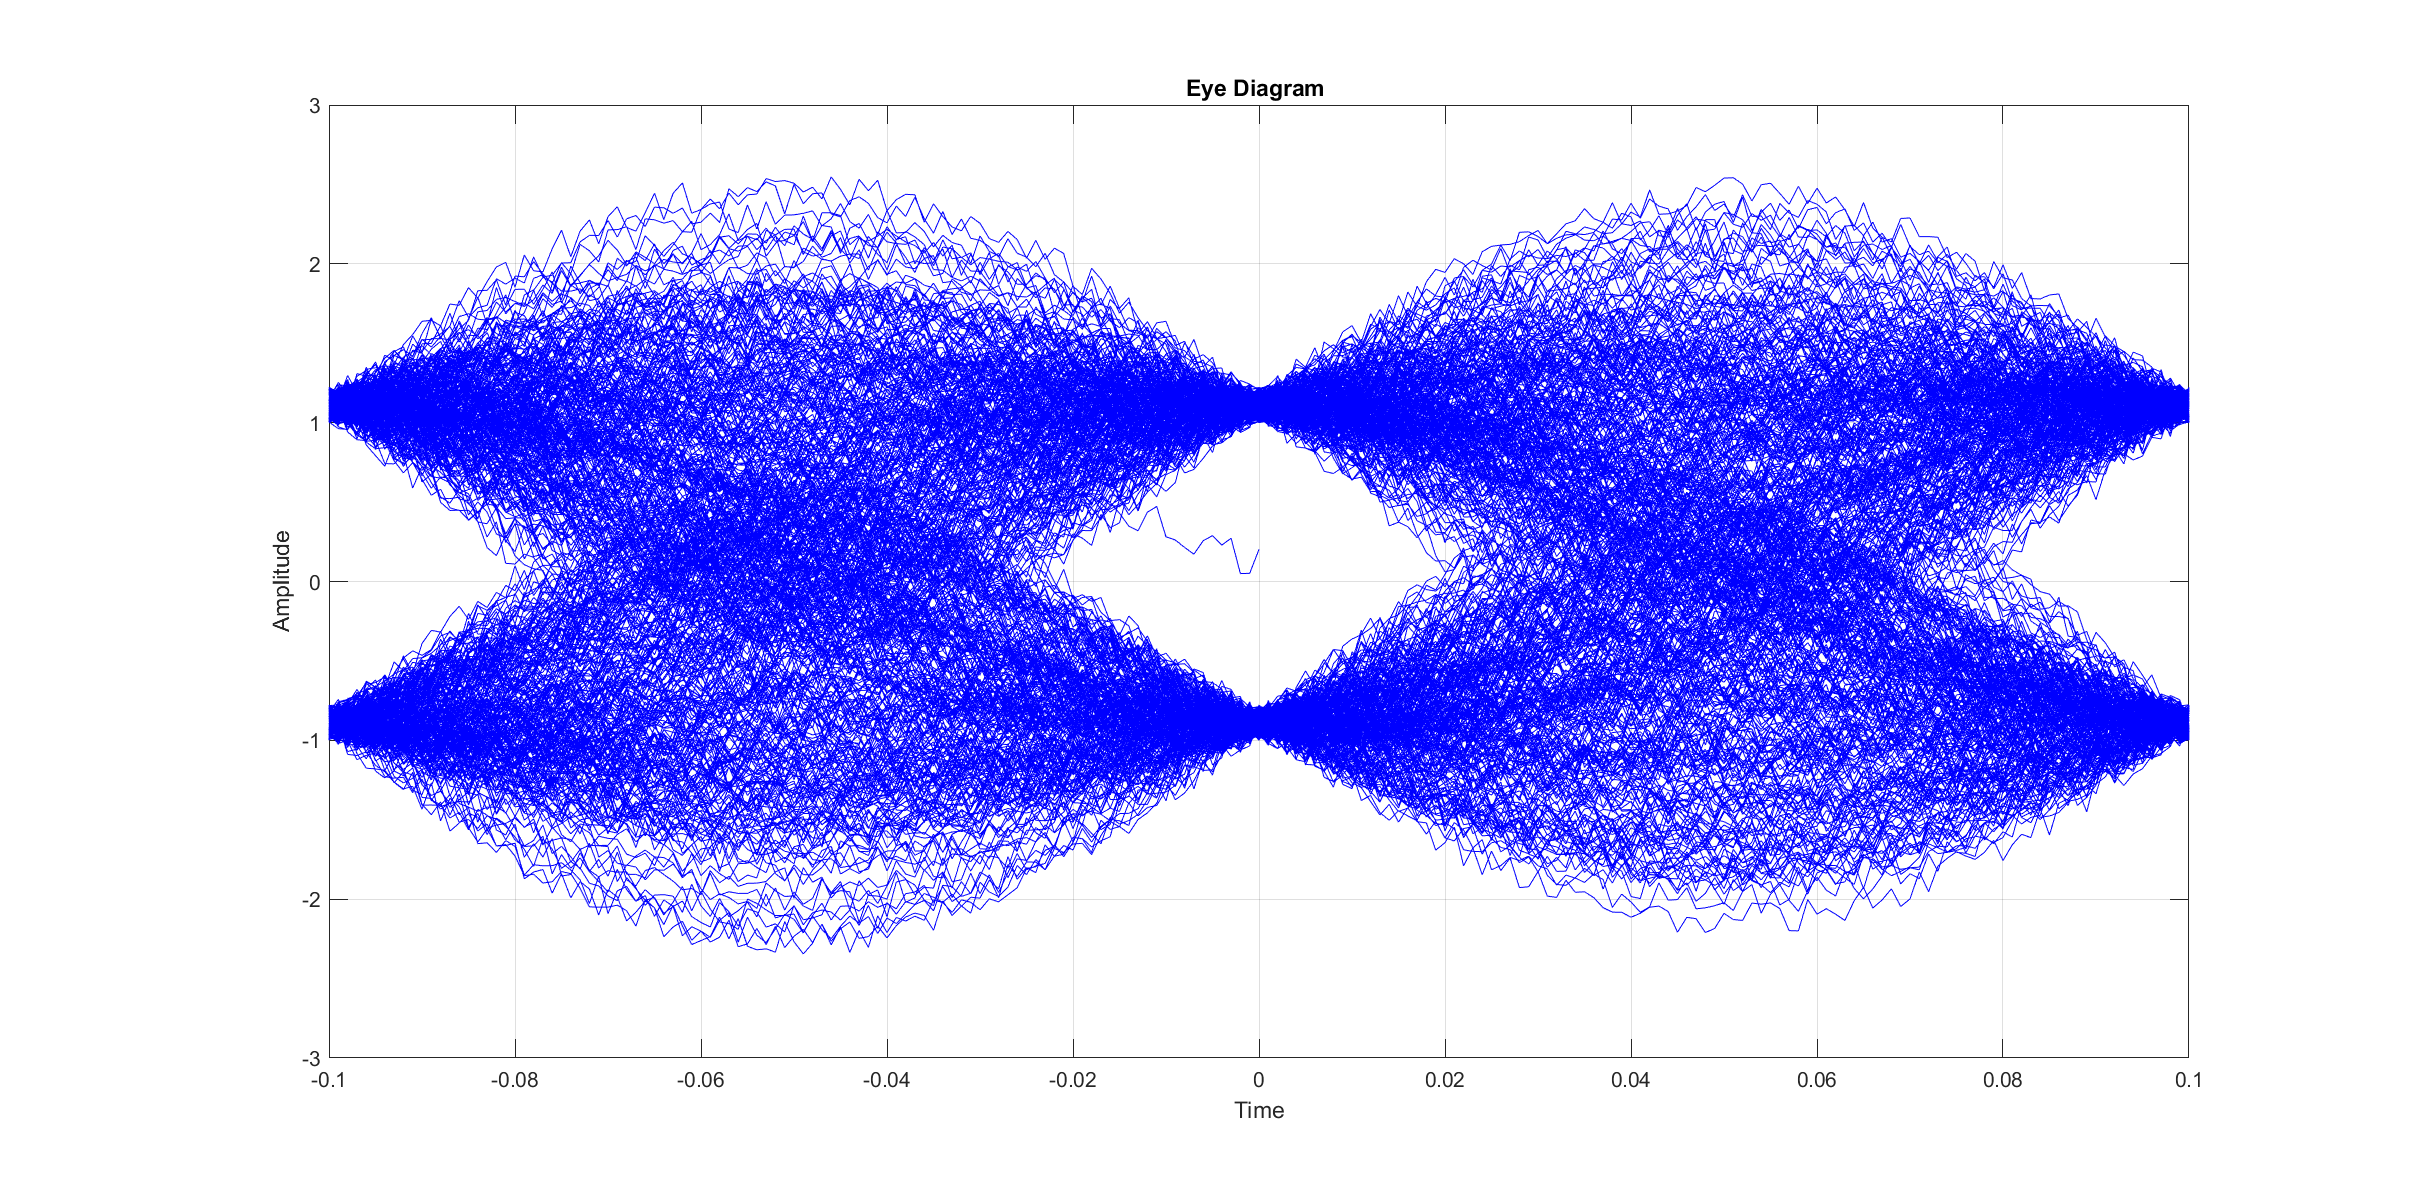
\includegraphics[scale=0.4]{figures/task22}
	\caption{Eye Diagram}
\end{figure}

\pagebreak
\subsection{Affect of AWGN, when using the Raised Cosine with with roll-off factor $\alpha = 0.5$ as the Impulse response}

\begin{figure}[H]
	\centering
	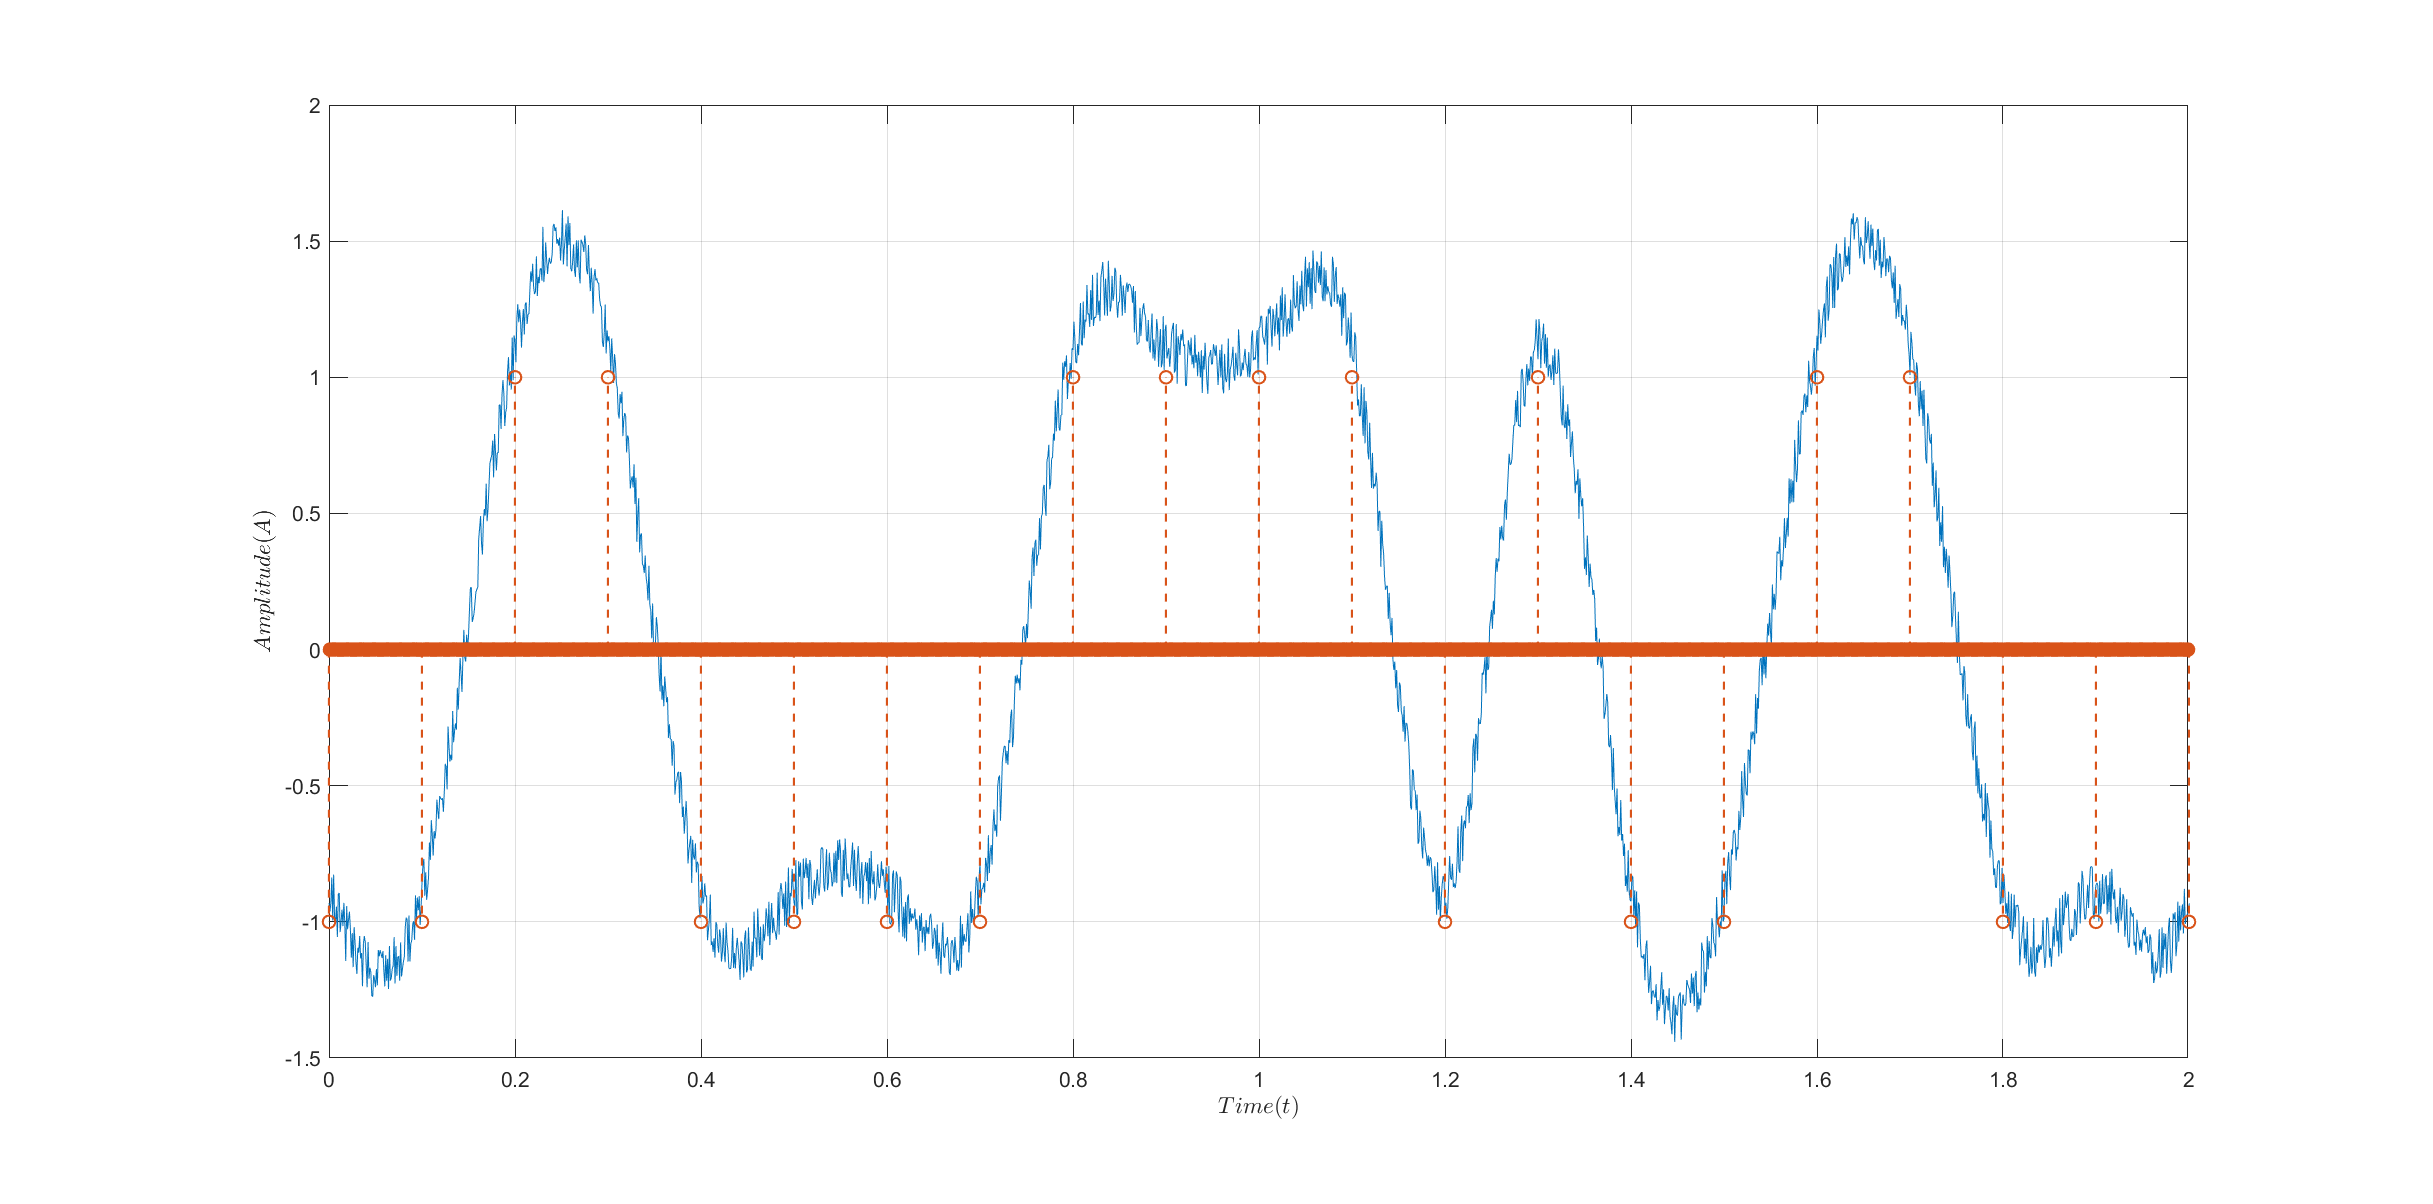
\includegraphics[scale=0.4]{figures/task23}
	\caption{Transmit Signal}
\end{figure}

\begin{figure}[H]
	\centering
	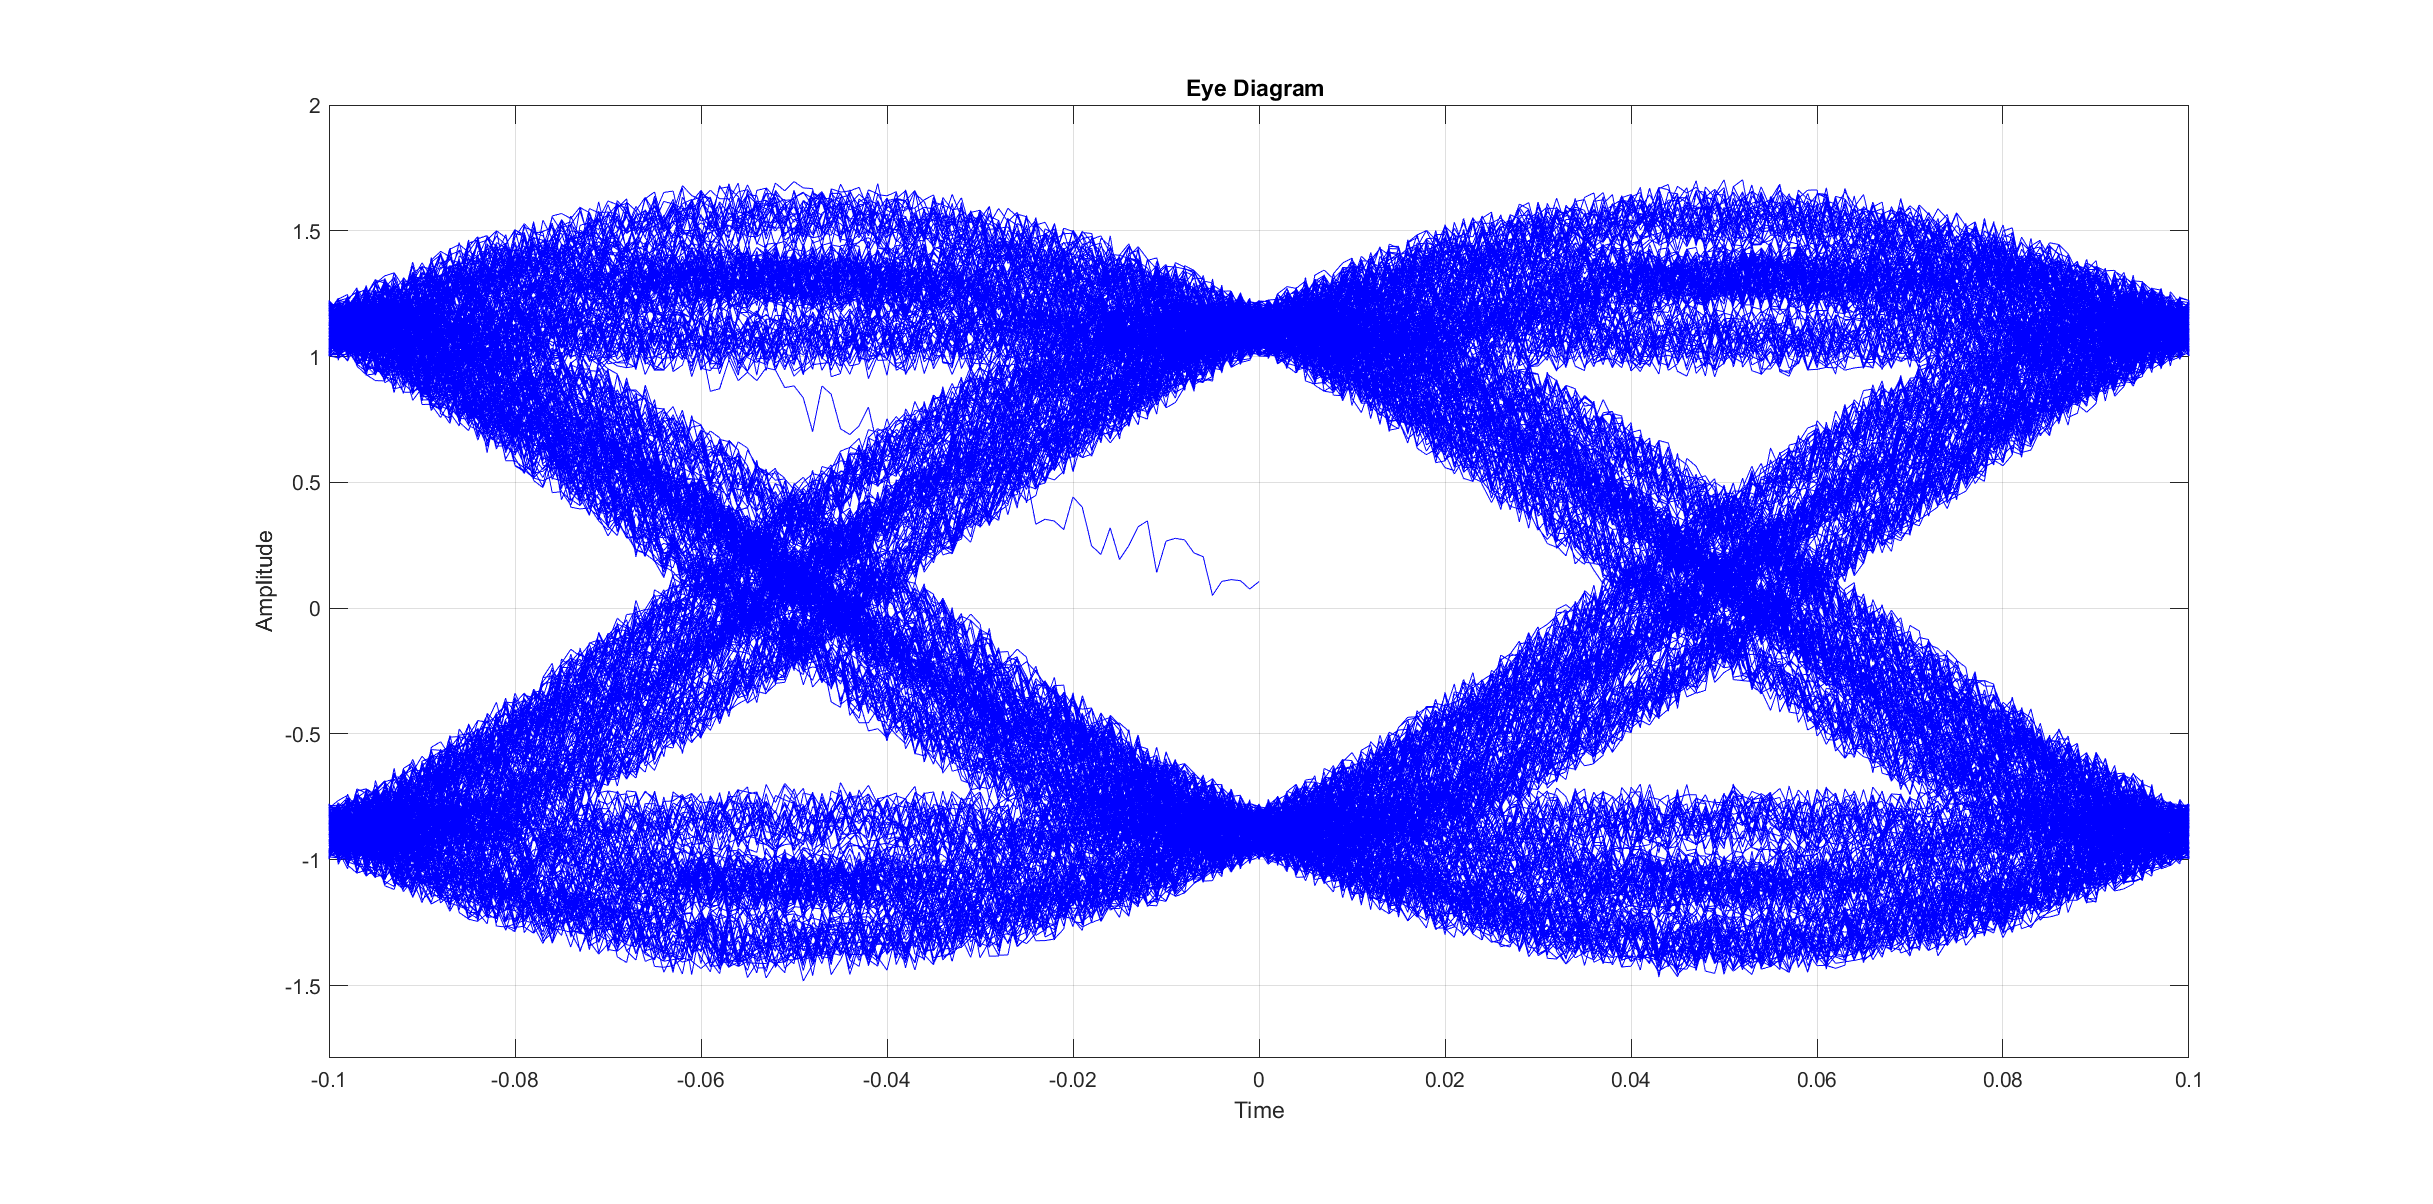
\includegraphics[scale=0.4]{figures/task24}
	\caption{Eye Diagram}
\end{figure}


\pagebreak
\subsection{Affect of AWGN, when using the Raised Cosine with with roll-off factor $\alpha = 1$ as the Impulse response}

\begin{figure}[H]
	\centering
	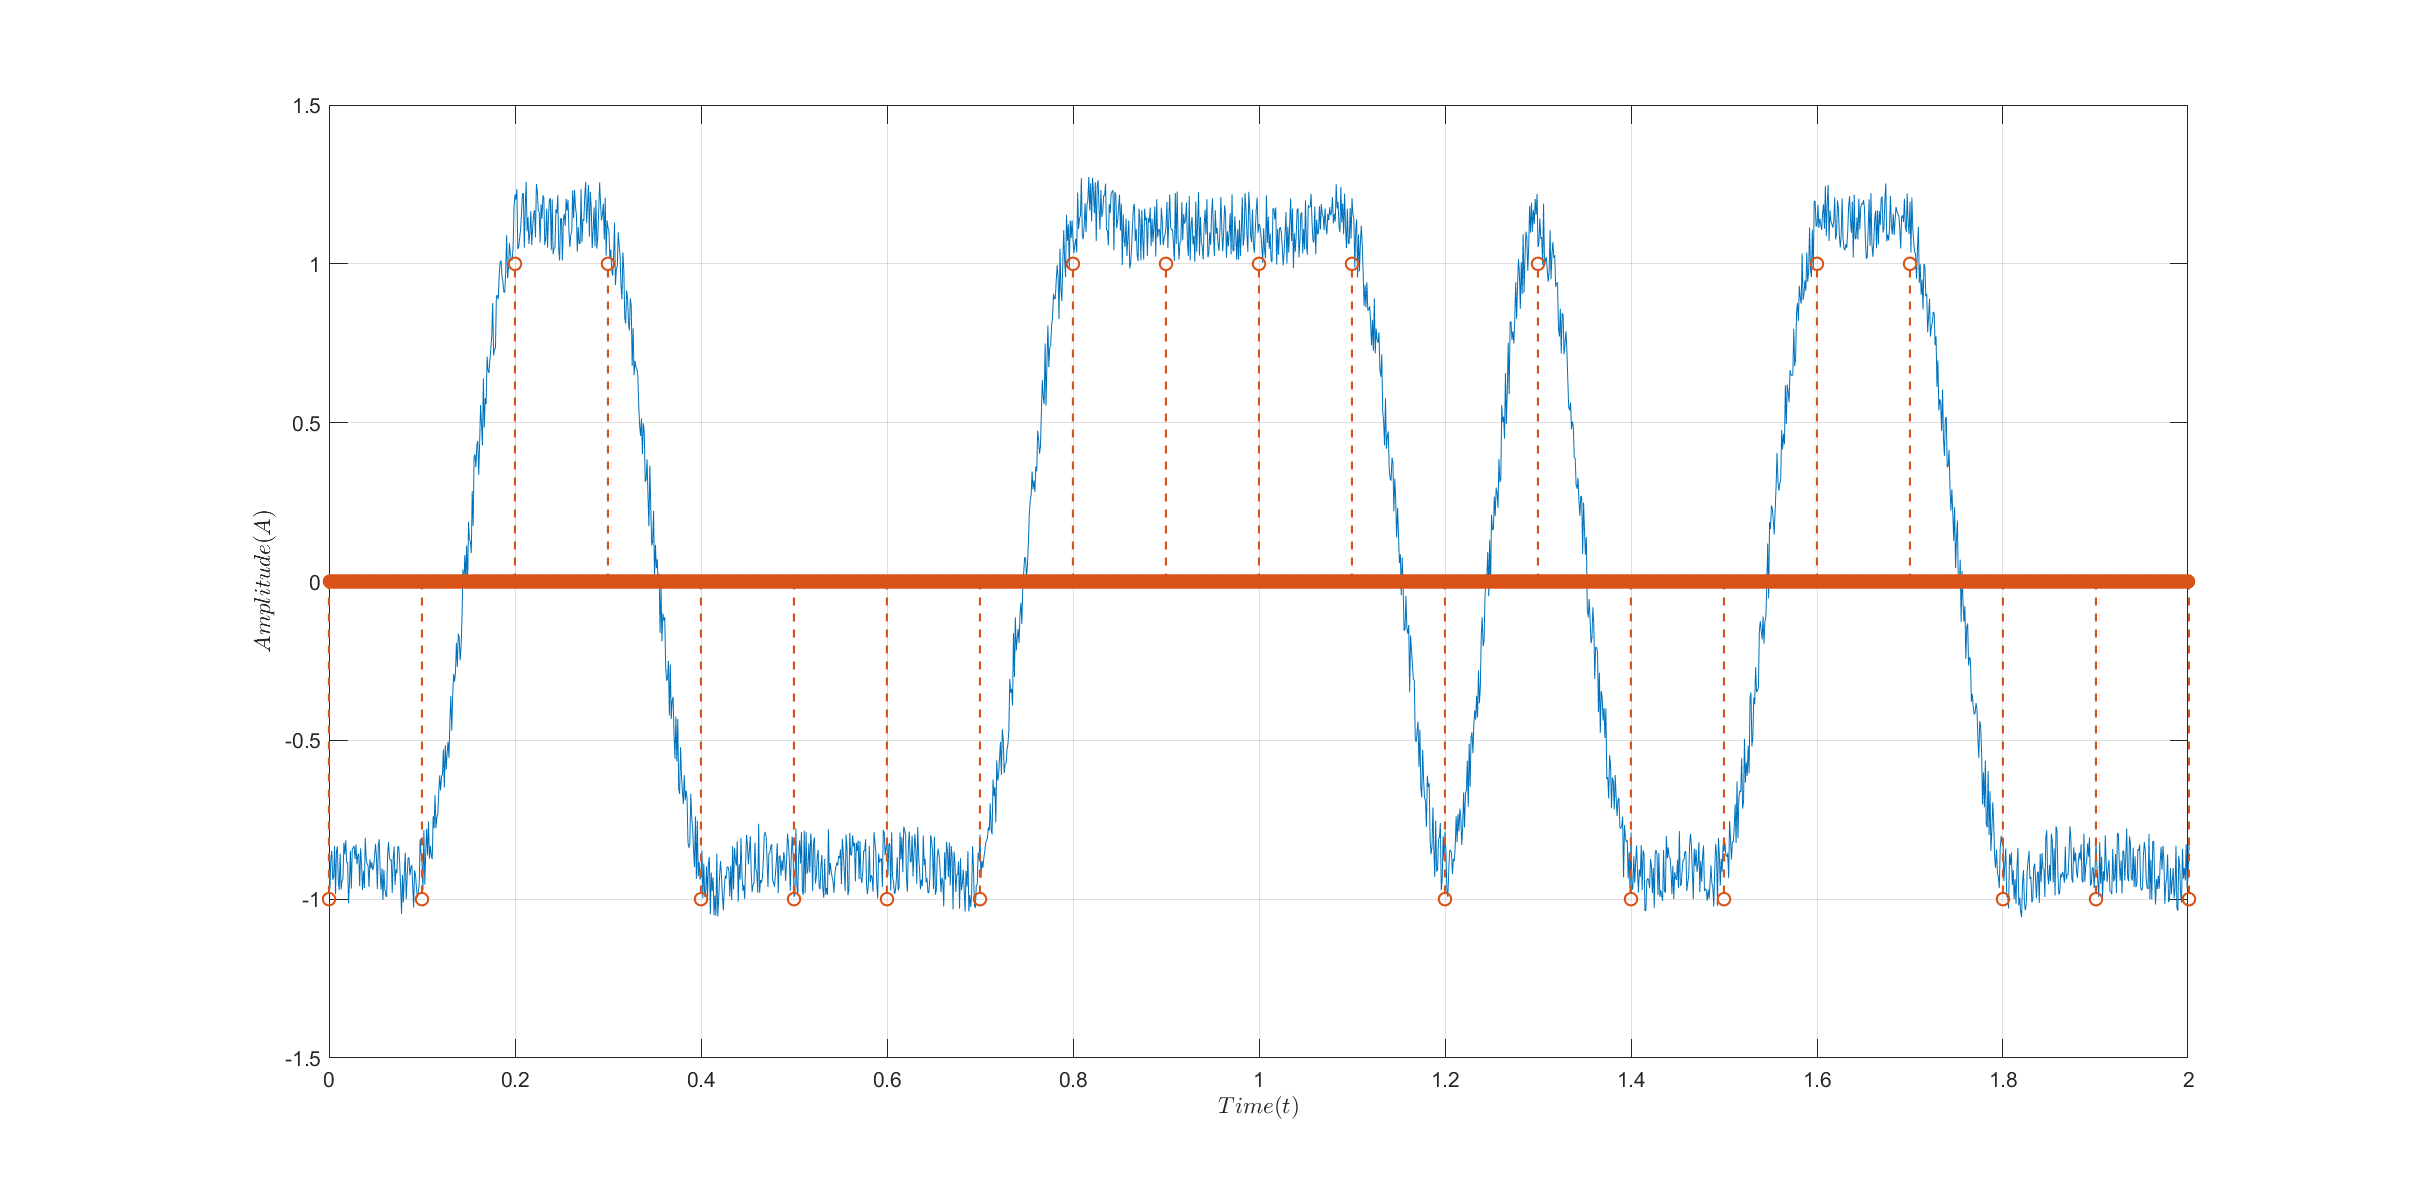
\includegraphics[scale=0.4]{figures/task25}
	\caption{Transmit Signal}
\end{figure}

\begin{figure}[H]
	\centering
	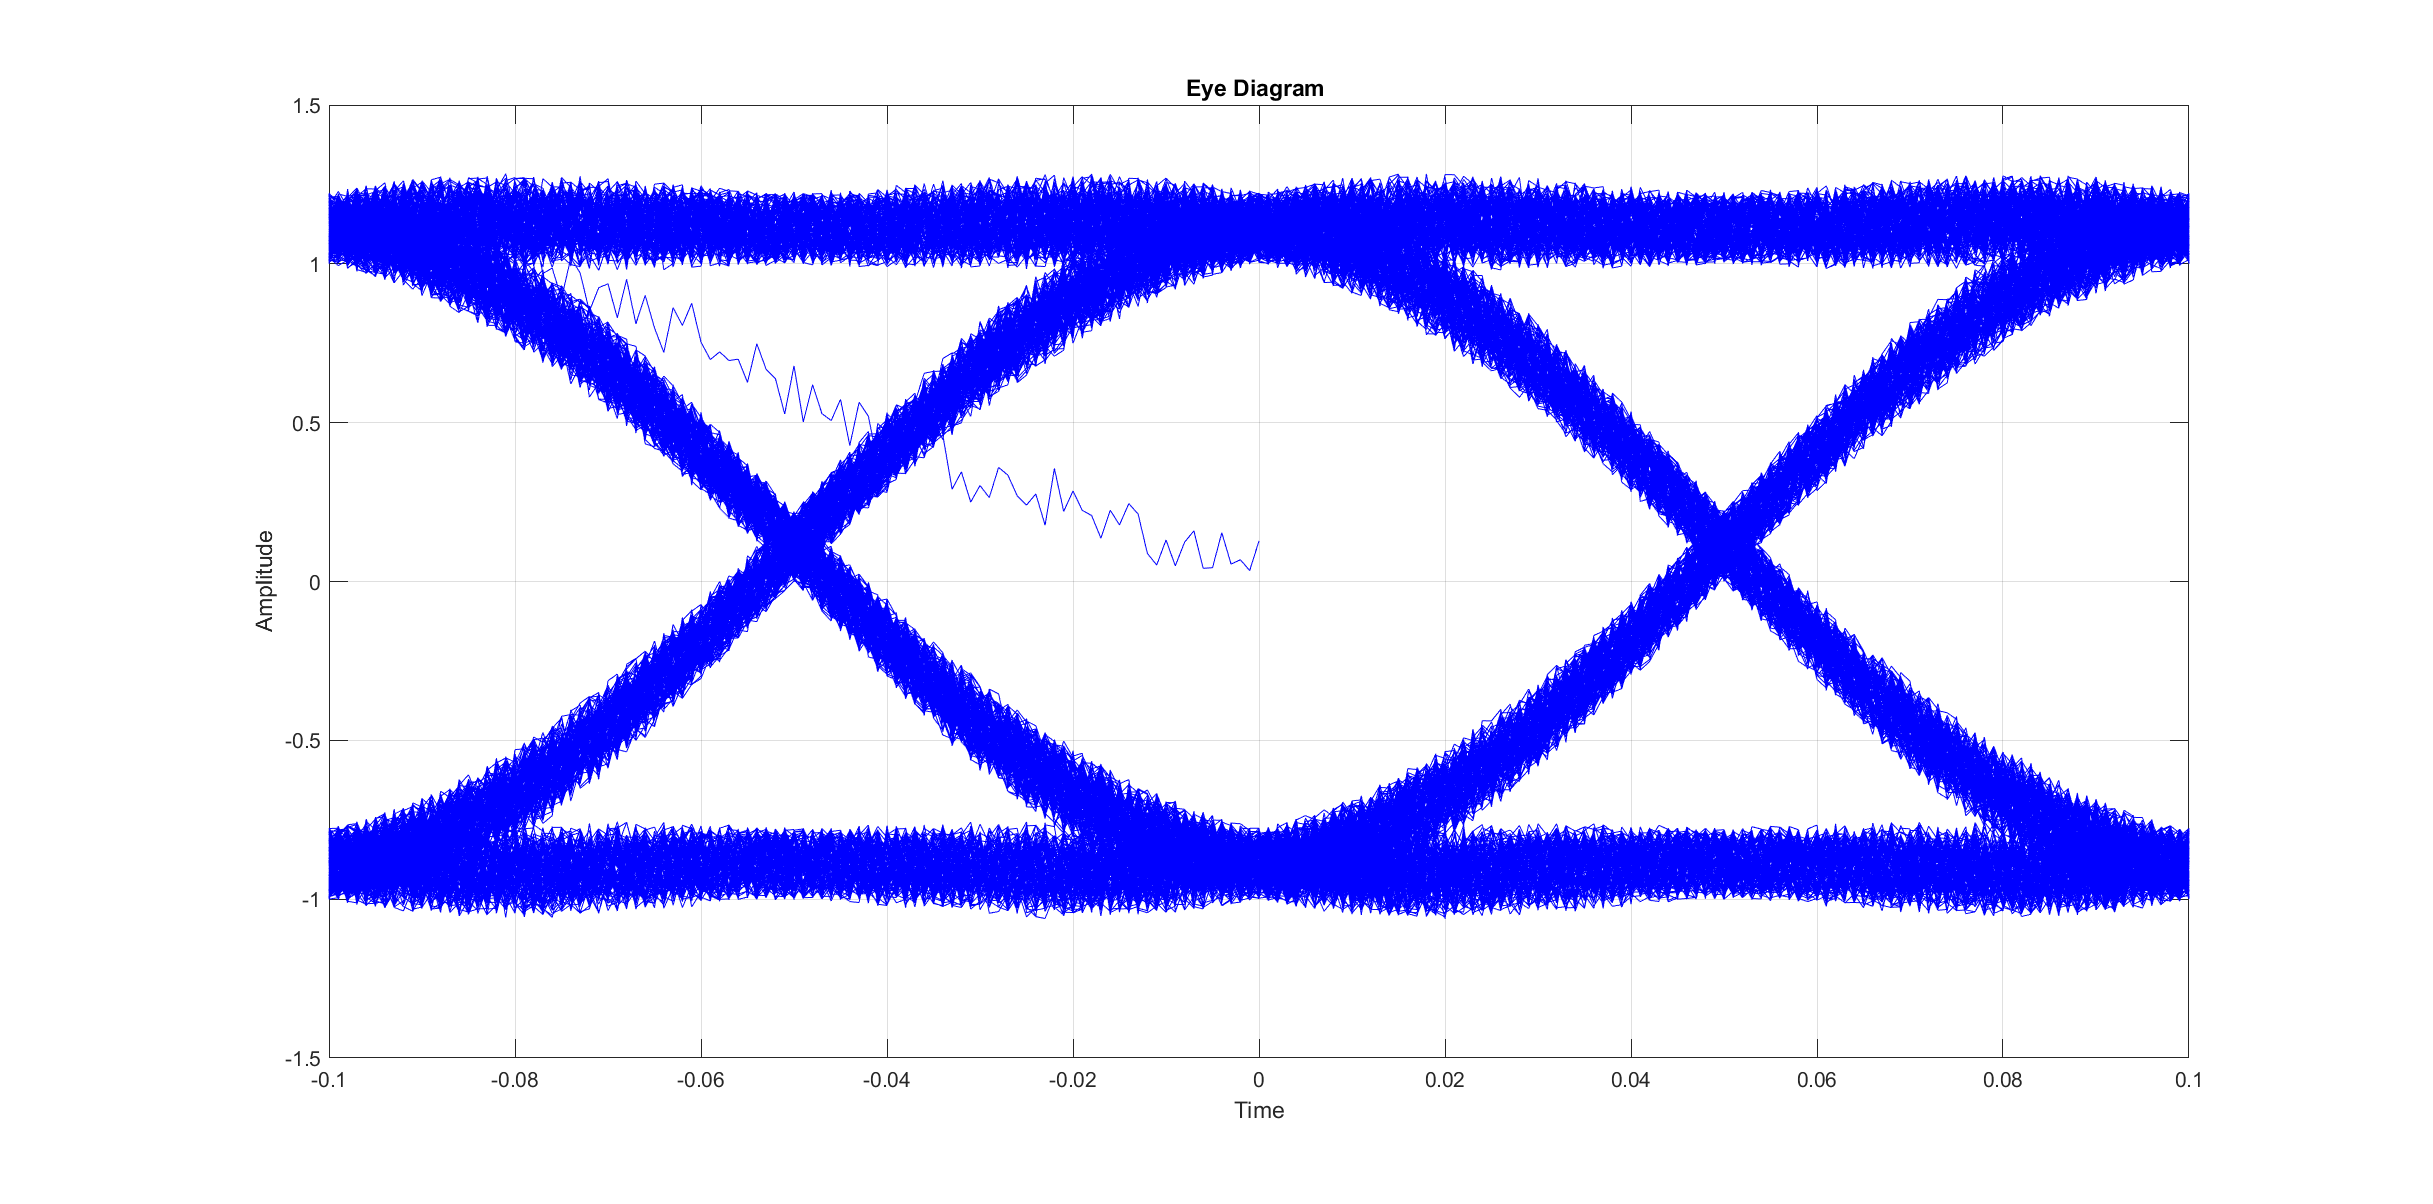
\includegraphics[scale=0.4]{figures/task26}
	\caption{Eye Diagram}
\end{figure}

\subsection{Robustness of the system with respect to noise, sampling time and synchronization errors}

Addition of AWGN has diminished the performance of all the three systems.This is clearly visible in all the three eye diagrams as that noise addition has made the eye smaller than the noise-free situation.

\begin{itemize}
	\item \textbf{Optimum Sampling Instant at maximum eye opening}: Systems has slight changes in the instance at maximum eye opening due to the added AWGN. 
	It's not the same as previous AWGN free situation.
	\item \textbf{Error-Free Sampling Region}: {\tt raised cosine} filter with  the higher roll-off factor still shows the widest error free sampling region. Whereas AWGN has reduced, that of {\tt sinc} filter in great amount. This makes the raised cosine filter more robust under the AWGN environment.
	\item \textbf{Level-Crossings at the corners of the eye}: As mentioned in the task 1 comparison, {\tt raised cosine} filter with  the higher roll-off factor has the narrowest level-crossing regions out of all the discussed systems. This makes that filter to be more robust for ISI, under the addition of the AWGN.
	
\end{itemize}

\section{Task 3}
\subsection{Question 1 - 10}
\begin{figure}[H]
	\centering
	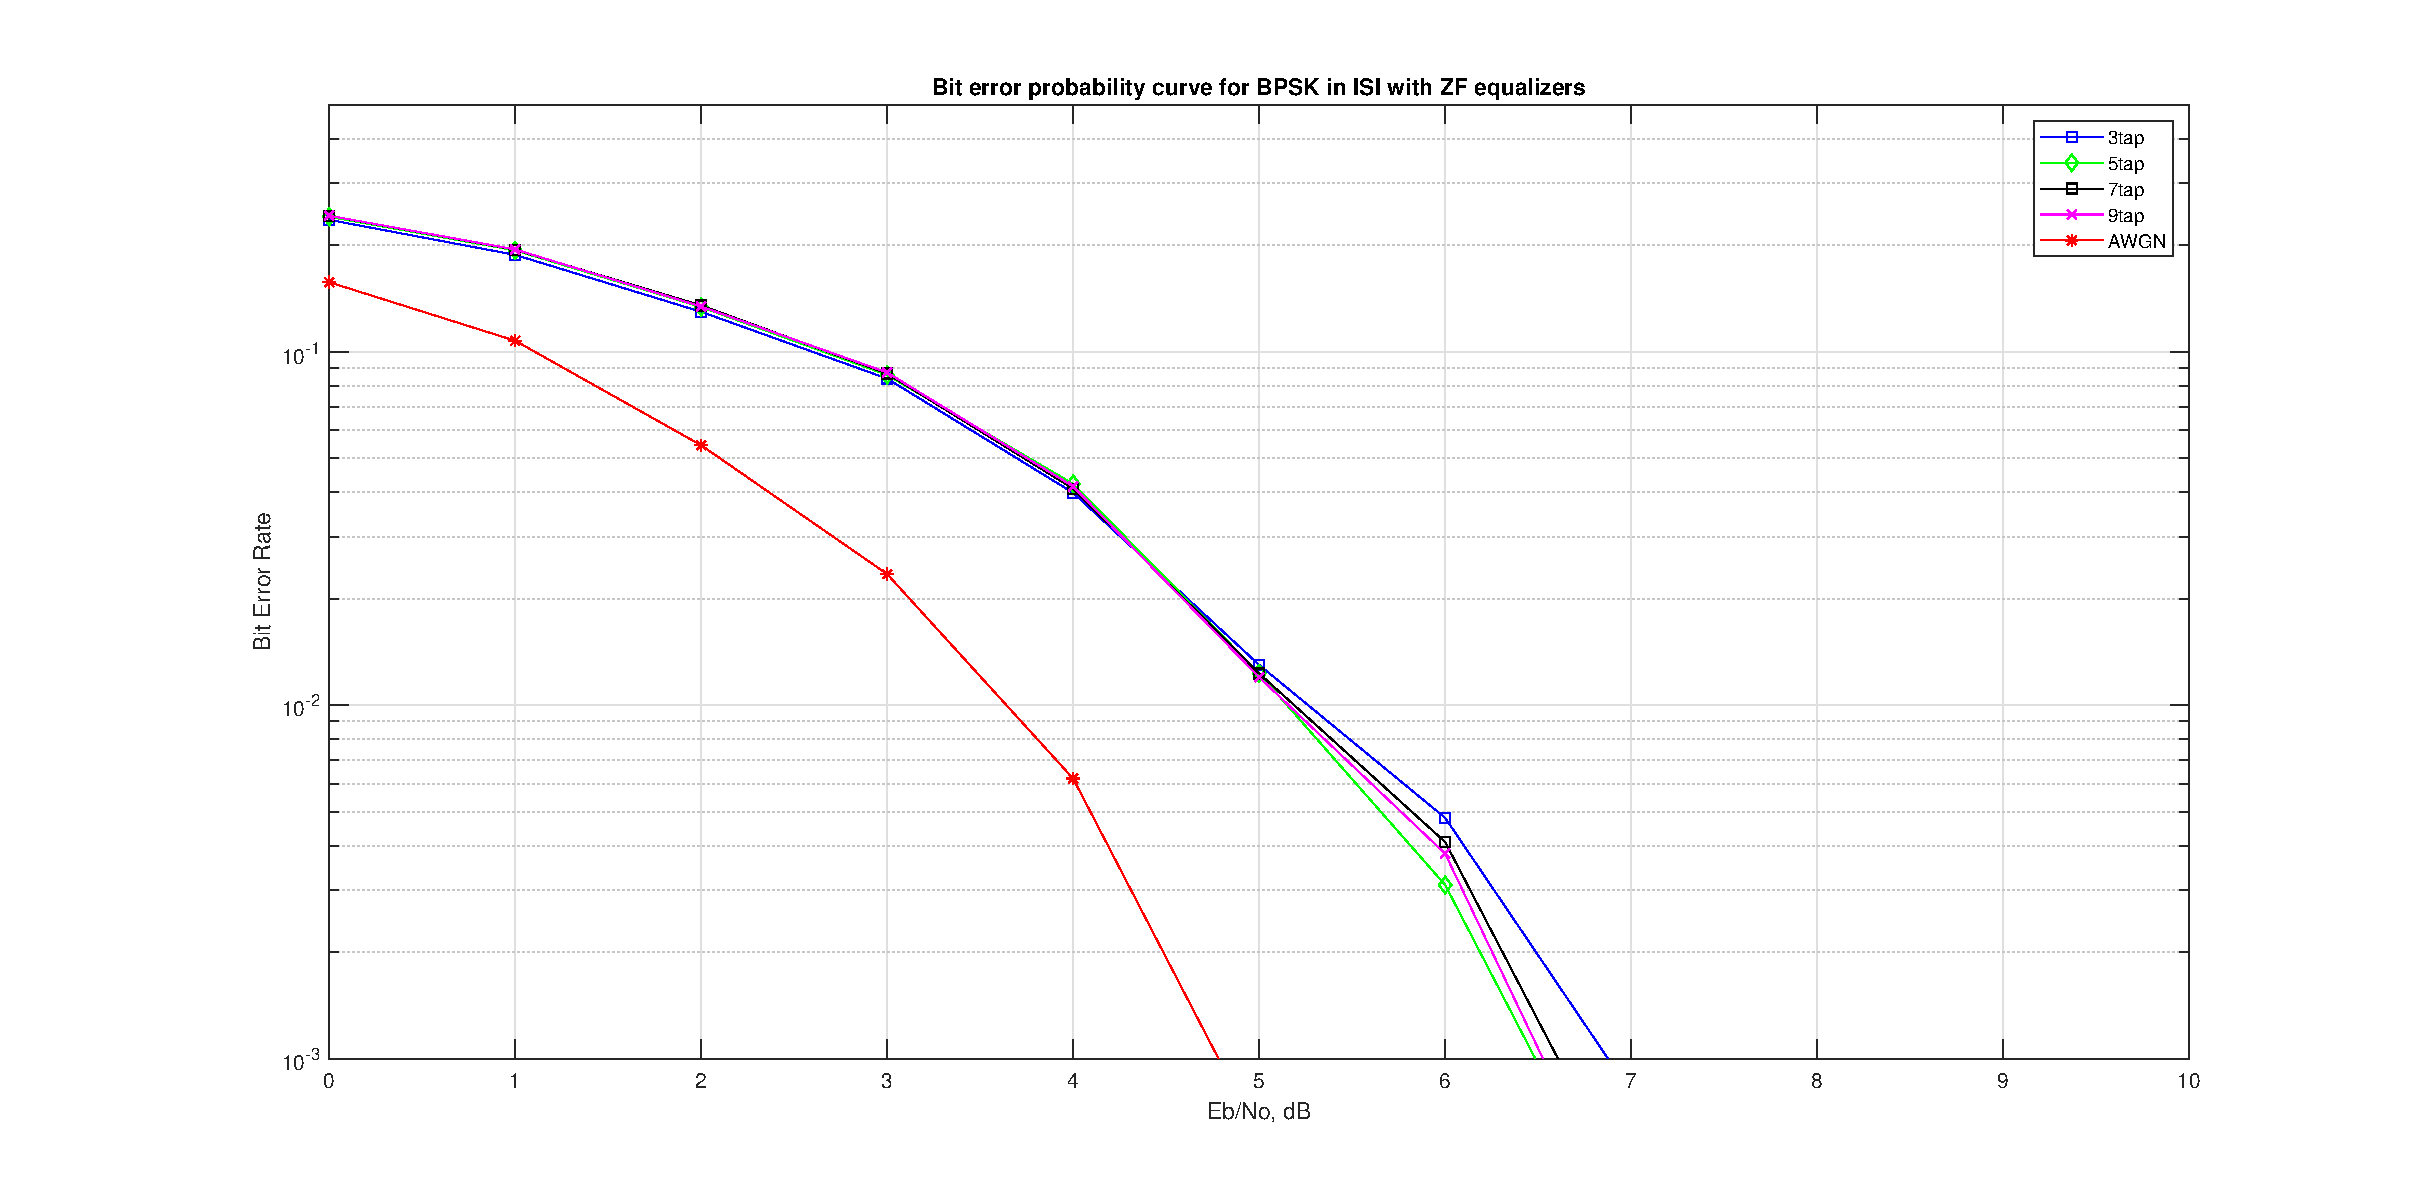
\includegraphics[scale=0.4]{figures/task31}
	\caption{Bit error probability curve for BPSK in ISI with ZF equalizers}
\end{figure}

\subsection{Question 11}
In the Zero force Equalizer multi-path channel noise also get amplified. So the bit error rate is high. Since there is no any amplification in the noise in AWGN channel BER is less than Zero force equalizer multi path channel.


\begin{appendices}
	\section{Matlab Code for the Implementation}
	\includepdf[pages=-, width=1.2\textwidth]{code/task.pdf}
\end{appendices}

%---------------------------------------------------------------------------
\end{document}
